\documentclass[oneside, 12pt]{book}
\usepackage{icdthesisUTF}
\usepackage{tabularx} 
\usepackage{epsfig}
\usepackage{listings}

\usepackage{color}
\renewcommand{\lstlistingname}{Αλγόριθμος}
\renewcommand{\lstlistlistingname}{Κατάλογος αλγορίθμων}
\definecolor{dkgreen}{rgb}{0,0.6,0}
\definecolor{gray}{rgb}{0.5,0.5,0.5}
\definecolor{mauve}{rgb}{0.58,0,0.82}

\lstset{frame=tb,
  language=Java,
  aboveskip=3mm,
  belowskip=3mm,
  showstringspaces=false,
  columns=flexible,
  basicstyle={\small\ttfamily},
  numbers=none,
  numberstyle=\tiny\color{gray},
  keywordstyle=\color{blue},
  commentstyle=\color{dkgreen},
  stringstyle=\color{mauve},
  breaklines=true,
  breakatwhitespace=true,
  tabsize=3,
  numbers=left,
  stepnumber=1,
  captionpos=b
}
%Τα παρακάτω είναι υποχρεωτικά:

\renewcommand{\thesistitle}{Ανάπτυξη εφαρμογής για την καταγραφή της μετακίνησης πληθυσμών με σκοπό την εξαγωγή πληροφοριών για πιθανές διαδρομές μετάδοσης ασθενειών }
\renewcommand{\thesisauthor}{Άντι Άσκο (3026)}
\renewcommand{\thesisauthorabbrv}{Α. Άσκο}
\renewcommand{\thesisauthorinitials}{ΑΑ}
\renewcommand{\thesissupervisor}{Δρ. Πεταλίδης Νικόλαος, Επιστημονικός Συνεργάτης}
\renewcommand{\thesismonth}{Φεβρουάριος}
\renewcommand{\thesisyear}{2018}

% Η βιβλιογραφία
\addbibresource{testUTF.bib}

\begin{document}
% Υποχρεωτικά τα παρακάτω:
\Titlepage
\Declarationpage
\begin{Abstract}
Επιδημία χαρακτηρίζεται η ταχεία μετάδοση μίας ασθένειας σε ένα μεγάλο αριθμό ατόμων σε ένα μικρό χρονικό διάστημα. Μια μικρή αναδρομή στο παρελθόν μας αποκαλύπτει ότι το ανθρώπινο είδος έχει βρεθεί ουκ ολίγες φορές αντιμέτωπο με διάφορες επιδημίες άλλες πιο επικίνδυνες και άλλες λιγότερες. Καθώς το ανθρώπινο είδος εξελίσσεται και η επιστήμη της ιατρικής έχει καταφέρει να απαλείψει ένα πολύ μεγάλο βαθμό ασθενειών, δεν παύουμε να βρισκόμαστε σε κίνδυνο νέων ασθενειών.
\par
Σκοπός της πτυχιακής αυτής είναι η διερεύνηση των δυνατοτήτων που μπορεί να προσφέρει η τεχνολογία και συγκεκριμένα τα μοντέρνα κινητά τηλέφωνα στην καταπολέμηση των επιδημιών, βοηθώντας στην εύρεση των ατόμων που ήρθαν σε επαφή με έναν φορέα.  Η πτυχιακή εστιάζει στην ανάπτυξη μιας εφαρμογής η οποία έχει τη δυνατότητα να καταγράφει τις διάφορες τοποθεσίες του χρήστη  καθώς και τη δυνατότητα να προειδοποιεί τους χρήστες σε περίπτωση που ήρθαν σε επαφή με κάποιον φορέα.
\end{Abstract}
\tableofcontents

%Μόνο εφόσον θέλετε χωριστό πίνακα για εικόνες και πίνακες
\listoftables
\listoffigures
\lstlistoflistings
% %Προαιρετικά
% \begin{Preface}


% \end{Preface}

%Προαιρετικά
\begin{Acknowledgement}
Η πτυχιακή μου εργασία είναι αφιερωμένη στους γονείς μου, Fatos και Majlinda, και την αδερφή μου Semi που με στήριξαν καθ’ όλη τη διάρκεια των φοιτητικών μου χρόνων και μη. Επίσης ευχαριστώ θερμά τον καθηγητή μου, κ. Νίκο Πεταλίδη για την γνώση που μου μετέφερε κατά την διάρκεια των φοιτητικών μου χρόνων όπως και την πολύτιμη βοήθεια του στην εξέλιξη μου ως επαγγελματίας.
\end{Acknowledgement}

%Προαιρετικά
% \begin{Definitions}
% \begin{description}
% \item [Cross Platform] Λογισμικό το οποίο τρέχει σε διαφορετικά λειτουργικά συστήματα ή πλατφόρμες υλικού

% \item [ReST API] Υπηρεσία η οποία προσφέρετε από μία συσκευή σε μία άλλη μέσω του διαδικτύου

% \item [RESTful] Υπηρεσία η οποία προσφέρετε από μία συσκευή σε μία άλλη μέσω του διαδικτύου


% \end{description}

% \end{Definitions}

\chapter{Εισαγωγή}
\leftmark\rightmark
\section{Γενικά}
Σε περίπτωση κρουσμάτων μιας μεταδιδόμενης ασθένειας, ένας από τους πρωταρχικούς στόχους των υπηρεσιών υγείας είναι η άμεση εύρεση των ατόμων που ήρθαν σε επαφή με έναν από τους φορείς ώστε να μειωθεί όσο το δυνατόν περισσότερο η μετάδοση σε περισσότερα άτομα. Δυστυχώς μία τέτοια διαδικασία εμφανίζει δυσκολίες. Πολλές φορές οι φορείς δεν θυμούνται τις ακριβείς τοποθεσίες στις οποίες βρέθηκαν με αποτέλεσμα να μην είναι δυνατή η εύρεση όλων των ατόμων με τους οποίους ήρθαν σε επαφή. 
\par
Επομένως ένα από τα μεγαλύτερα προβλήματα που εμφανίζονται είναι η αδυναμία των φορέων να ξαναφέρουν στη μνήμη τους όλα τα άτομα με τα οποία ήρθαν σε επαφή τις τελευταίες μέρες. Επιπλέον ένα ακόμη μεγάλο πρόβλημα που αντιμετωπίζουν οι υπηρεσίες υγείας είναι η αδυναμία να επικοινωνήσουν με τα άτομα που ήρθαν σε επαφή με έναν φορέα ώστε να τους προειδοποιήσουν. Ως εκ τούτου δημιουργείται η ανάγκη εύρεσης μια λύσης στα παραπάνω προβλήματα. 

\section{Στόχοι της εργασίας}
Η πτυχιακή επικεντρώνεται στην εύρεση τρόπων με τους οποίους οι νέες τεχνολογίες και συσκευές θα μπορούσαν να βοηθήσουν τις υπηρεσίες υγείας στην επίλυση των παραπάνω προβλημάτων. Εστιάζει στις δυνατότητες που προσφέρουν οι καινούριες κινητές συσκευές στην παρακολούθηση και καταγραφή των τοποθεσιών στις οποίες βρέθηκε ο χρήστης όπως επίσης και στην δυνατότητα της συνεχής πρόσβασης στο διαδίκτυο και ως εκ τούτου την ικανότητα άμεσης ενημέρωσης του.

\section{Δομή της εργασίας}
Η εργασία χωρίζεται σε επτά κεφάλαια. Αρχικά, στο επόμενο κεφάλαιο, θα υπάρξει μια θεωρητική ανάλυση των διάφορων εννοιών και τεχνολογιών που θα χρησιμοποιήθηκαν για την ανάπτυξη της πτυχιακής εργασίας. Έπειτα, θα παρουσιαστούν οι περιπτώσεις χρήσης του συστήματος. Αμέσως μετά, θα υπάρξει μια πλήρης περιγραφή του συστήματος στα διάφορα μέρη τα οποία το απαρτίζουν. Κατόπιν, θα παρουσιαστεί ο τρόπος υλοποίησης των διάφορων επιπέδων, καθώς επίσης θα αναλυθούν τα επιμέρους τεχνικά κομμάτια. Στη συνέχεια, θα παρουσιάσουμε τους τρόπους με τους οποίους έγινε ο έλεγχος ποιότητας του έργου. Τέλος, θα παρουσιαστούν τα διάφορα συμπεράσματα στα οποία καταλήξαμε καθώς και οι προτάσεις εξέλιξης του συστήματος.	
\chapter{Θεωρητική ανάλυση}

\section{Εισαγωγή}
Σε αυτό το κεφάλαιο θα γίνει μια σύντομη ανάλυση εννοιών οι οποίες είναι αναγκαίο να γίνουν κατανοητές προτού εισέλθουμε σε λεπτομερείς ανάλυση της πτυχιακής εργασίας. Επιπλέον, θα γίνει σύντομη ανάλυση των απαιτήσεων για την επίτευξη της πτυχιακής όπως επίσης και των εργαλείων που χρησιμοποιήθηκαν. 

\section{Ανάπτυξη εφαρμογών κινητών συσκευών}
Όπως είναι γνωστό, η εξέλιξη της τεχνολογίας στο τομέα των κινητών συσκευών είναι ραγδαία τα τελευταία χρόνια με αποτέλεσμα οι δυνατότητες τους συνεχώς να επεκτείνονται. Πλέον μια συσκευή παρέχει στο χρήστη δυνατότητες αντάξιες ενός υπολογιστή σε ένα αισθητά πολύ μικρότερο μέγεθος. Εδώ θα πρέπει να σημειώσουμε ότι ο όρος κινητές συσκευές δεν διαχωρίζει τις τηλεφωνικές συσκευές από τα tablet καθώς ο διαχωρισμός μεταξύ τους, την σήμερον ημέρα, γίνεται όλο και πιο δύσκολος. Παρακάτω θα αναλύσουμε τις εφαρμογές κινητών συσκευών, την ιστορική αναδρομή των τελευταίων ετών καθώς και τις κύριες πλατφόρμες που βρίσκονται αυτή τη στιγμή στην αγορά. Επίσης θα αναλύσουμε τα προβλήματα τα οποία εμφανίζει η σημερινή αγορά κινητών συσκευών σε έναν προγραμματιστή και τις λύσεις που προσφέρονται.

\subsection{Εξέλιξη στον τομέα των κινητών συσκευών}
Οι κινητές συσκευές είχαν μια συνεχή εξέλιξη από τις αρχές του 2000 με καινούριες δυνατότητες να προστίθενται συνεχώς και η λειτουργικότητα τους να αυξάνεται αισθητά. Εάν επικεντρωθούμε στα νεότερα χρόνια, Από την εμφάνιση του πρώτου iPhone το 2007 της εταιρείας Αpple η οποία έκανε το πρώτα βήματα στον κόσμο των έξυπνων τηλεφώνων (smartphones), μέχρι την εμφάνιση του android λειτουργικού συστήματος μπορούμε να παρατηρήσουμε πως οι κατασκευάστριες εταιρείες επικεντρώνονται όλο και περισσότερο στην αύξηση των δυνατοτήτων που μπορεί να προσφέρει μια κινητή συσκευή. 
\par
Εν έτη 2018 μία απλή κινητή συσκευή έχει εξίσου τις ίδιες δυνατότητες με έναν ηλεκτρονικό υπολογιστή. Ο χρήστης έχει τη δυνατότητα σύνδεσης στο διαδίκτυο, την χρήση πολύπλοκων εφαρμογών όπως λογισμικά επεξεργασίας κειμένου μέχρι τη χρήση εφαρμογών GPS για τη καθοδήγηση του. Θα τολμούσαμε να πούμε πως καθημερινά το χάσμα μεταξύ των ηλεκτρονικών υπολογιστών και των κινητών συσκευών γίνεται όλο και μικρότερο.

\subsection{Πλατφόρμες κινητών συσκευών}
Ακολουθώντας την εξέλιξη στις κινητές συσκευές, παρατηρούμε ότι διάφορες πλατφόρμες και λειτουργικά συστήματα έχουν κάνει την εμφάνιση τους. Σκοπός της εργασίας αυτής δεν είναι να αναλύσει τις διάφορες πλατφόρμες, παρόλα αυτά είναι αναγκαία η παρουσίαση τους στον αναγνώστη για την περαιτέρω κατανόηση της ανάπτυξης της εφαρμογής. Σήμερα οι μεγαλύτερες πλατφόρμες κινητών συσκευών στην αγορά είναι τρεις:

\begin{description}
\item [iOs] Είναι το λειτουργικό σύστημα στις συσκευές iphone και ipad της εταιρείας Apple.

\item [Windows phone] Είναι το λειτουργικό σύστημα της εταιρείας Microsoft. Κάνει την εμφάνιση του κυρίως στις συσκευές της εταιρείας Nokia.

\item [Android] Είναι το λειτουργικό σύστημα ανοιχτού κώδικα της εταιρείας Google. Εμφανίζεται σε διάφορες συσκευές διάφωρων εταιρειών. Θεωρείται το κυρίαρχο λειτουργικό σύστημα στην αγορά εργασίας.
\end{description}

\par
Φυσικά υπάρχει ένα αξιοσέβαστος αριθμός άλλων λειτουργικών συστημάτων που έχουν κάποιο μερίδιο στην αγορά. Η παραπάνω επιγραμματική παρουσίαση έχεις ως στόχο να προσφέρει στον αναγνώστη μια μικρή εισαγωγή στο πρόβλημα που αντιμετωπίζουν οι προγραμματιστές εφαρμογών κινητών συσκευών. Κάθε πλατφόρμα χρησιμοποιεί διαφορετικές γλώσσες προγραμματισμού με αποτέλεσμα η ανάπτυξη εφαρμογών να είναι ένα καίριο ζήτημα για τον προγραμματιστή. Με ποιον τρόπο επιλέγεις την πλατφόρμα ανάπτυξης και αν θελήσεις να υποστηρίξεις περισσότερο από μία, ποιο θα είναι το κόστος ανάπτυξης όπως επίσης και το κόστος συντήρησης;

\subsection{Υβριδικές εφαρμογές}
Καθώς οι διάφορες πλατφόρμες εξελίσσονται συνεχώς, αυτομάτως, καθίσταται μεγάλη πρόκληση η ανάπτυξη μιας εφαρμογής συμβατή με όλα τα διαφορετικά λειτουργικά συστήματα. Στην πραγματικότητα ο προγραμματιστής είναι αναγκασμένος να αναπτύξει την ίδια εφαρμογή πολλαπλές φορές. Αυτομάτως αυτή η κατάσταση αυξάνει το κόστος συντήρησης ακόμη και μιας απλής εφαρμογής.
\par 
Για την αντιμετώπιση του παραπάνω προβλήματος δημιουργήθηκαν κατάλληλα εργαλεία τα οποία προσφέρουν στον προγραμματιστή τη δυνατότητα ανάπτυξης της εφαρμογής μια φορά και να τη καθιστά συμβατή με τις περισσότερες κυρίαρχες πλατφόρμες. Ένα εργαλείο το οποίο προσφέρει αυτές τις δυνατότητες είναι το Apache Cordova framework. 

\subsubsection{Apache Cordova}
Κάνοντας χρήση του Cordova framework, o προγραμματιστής αναπτύσσει την εφαρμογή του με τεχνολογίες διαδικτύου όπως HTML, CSS, JavaScript. Η πλατφόρμα Cordova δίνει στο προγραμματιστή πρόσβαση στις δυνατότητες της κάθε συσκευής (κάμερα, GPS κ.τ.λ), ανεξαρτήτων λειτουργικού συστήματος, μέσα από μια ενοποιημένη διεπαφή \citep{Cordova} \citep{CordovaWiki}. Έτσι η εφαρμογή μπορεί να εκτελεστεί στα διάφορα λειτουργικά συστήματα. Παρόλα αυτά το Cordova framework έχει σαν μοναδικό στόχο τον παραπάνω, με αποτέλεσμα να μην ασχολείται καθόλου με την αισθητική και εμφάνιση της εφαρμογής.

\subsubsection{Ionic Framework}
Το Ionic framework προσφέρει στο προγραμματιστή τα απαραίτητα εξαρτήματα για τη δημιουργία μιας διεπαφής χρήστη η οποία ακολουθεί τα πρότυπα κάθε πλατφόρμας \citep{Ionic} \citep{IonicWiki}. Με αυτό το τρόπο ο προγραμματιστής σχεδιάζει τη διεπαφή χρήστη με αισθητική αποδεκτή από όλους τους χρήστες ανεξαρτήτως της πλατφόρμας επιλογής τους.

\subsubsection{Cordova \& Ionic}
Ο συνδυασμός των Cordova και Ionic frameworks προσφέρει στο προγραμματιστή ένα πλήρες σύστημα για τη δημιουργία υβριδικών εφαρμογών. Εδώ να σημειώσουμε πως τα παραπάνω εργαλεία δεν είναι τα μοναδικά στην αγορά, παρόλα αυτά θεωρούνται τα πιο ώριμα και προσφέρουν περισσότερες δυνατότητες σε σύγκριση με άλλα.

\section{Ανάπτυξη εφαρμογών διαδικτύου}
Οι ιστοσελίδες πλέον δεν παρουσιάζουν απλά ένα στατικό περιεχόμενο αλλά προσφέρουν στο χρήστη διαδραστικό περιεχόμενο. Η ραγδαία αύξηση των χρηστών στο χώρο του διαδικτύου δημιούργησε την ανάγκη ανάπτυξης προηγμένων ιστοσελίδων οι οποίες προσφέρουν στους χρήστες περισσότερες και πιο σύνθετες δυνατότητες. Σταδιακά όλες οι υπηρεσίες μεταφέρονται στο διαδίκτυο. Από ηλεκτρονικά καταστήματα αγορών μέχρι πολυσύνθετες εφαρμογές όπως κρατικές υπηρεσίες. Το φαινόμενο αυτό είχε ως αποτέλεσμα την ανάγκη νέων εργαλείων τα οποία μπορούν να προσφέρουν στο προγραμματιστή τη δυνατότητα ανάπτυξης αυτού του είδους εφαρμογών. Ένα από τα πιο ισχυρά εργαλεία στην αγορά είναι το AngularJS framework.

\subsubsection{AngularJS Framework}
Το AngularJS framework είναι ένα εργαλείο κατασκευής εφαρμογών διαδικτύου. Προσφέρει στον προγραμματιστή τη δυνατότητα να χειριστεί το περιεχόμενο της εφαρμογής του με δυναμικό τρόπο \citep{AngularJS} \citep{AngularJSWiki}. Με αυτό το τρόπο ο προγραμματιστής μπορεί να κατασκευάσει μία εφαρμογή διαδικτύου που είναι ικανή να προσφέρει τις ίδιες δυνατότητες με μία εφαρμογή ηλεκτρονικών υπολογιστών.

\section{Web Services}
Web Service είναι μια υπηρεσία η οποία είναι προσβάσιμη μέσω του διαδικτύου με στόχο την εξυπηρέτηση των χρηστών της ή άλλων εφαρμογών. Το web service καταστεί δυνατή την επικοινωνία διαφορετικών πελατών μέσω του HTTP πρωτοκόλλου. To web service προσφέρει πρόσβαση στις υπηρεσίες του μέσω ενός API. Η επικοινωνία γίνεται μέσω αιτήσεων, δηλαδή ο πελάτης ζητάει κάτι, το web service επεξεργάζεται το αίτημα και επιστρέφει την κατάλληλη απάντηση. Τα σύγχρονα web services χρησιμοποιούν την αρχιτεκτονική ReST για την υλοποίηση των API τους.

\begin{figure}[h]
  \centering
  \includegraphics[width=110mm]{images/web-service.png}
  \caption{Παράδειγμα Επικοινωνίας web service}
  \label{fig:web-service}
\end{figure}

\subsection{ReST API}
Όπως αναφέραμε παραπάνω το ReST είναι μία αρχιτεκτονική σχεδιασμού και υλοποίησης διεπαφών μεταξύ πελατών και web services. Χρησιμοποιεί το πρωτόκολλο HTTP ως δίαυλο επικοινωνίας. Λειτουργεί ανεξαρτήτως πλατφόρμας και γλώσσας προγραμματισμού οπότε καθιστά δυνατή την εξυπηρέτηση διαφορετικών πελατών. Η αρχιτεκτονική ReST βασίζεται σε 6 βασικές αρχές \citep{ReST}:

\subsubsection{Πελάτη-Εξυπηρετητή}
Το σύστημα είναι της μορφής πελάτη-εξυπηρετητή. Οι πελάτες είναι υπεύθυνοι για την εκκίνηση της επικοινωνίας καθώς ο εξυπηρετητής περιμένει για αιτήματα. Με αυτό το τρόπο οι ρόλοι διαχωρίζονται και η επικοινωνιακές αρχές είναι διακριτές.

\subsubsection{Πολυεπίπεδο σύστημα}
Το σύστημα διαχωρίζεται σε πολλαπλά επίπεδα με το κάθε επίπεδο να εξυπηρετεί το αμέσως επόμενο. Έτσι τα διάφορα επίπεδα παραμένουν αόρατα μεταξύ τους και το κάθε επίπεδο γνωρίζει μονάχα για το αμέσως επόμενο. 

\subsubsection{Stateless}
Κάθε αίτημα πρέπει να είναι ανεξάρτητο. Ο πελάτης είναι υπεύθυνος να προσφέρει όλες τις απαιτούμενες πληροφορίες στο εξυπηρετητή σε κάθε αίτημα του. Με αυτό το τρόπο ο εξυπηρετητής προσφέρει τις υπηρεσίες του ανεξαρτήτως άλλων αιτήσεων.

\subsubsection{Cacheable}
Το κάθε επίπεδο έχει τη δυνατότητα αποθήκευσης στη μνήμη οποιασδήποτε απάντησης έχει λάβει από κάποιο άλλο επίπεδο. Έτσι ο όγκος δεδομένων ελαττώνεται σημαντικά.

\subsubsection{Code on demand}
Ο πελάτης έχει τη δυνατότητα να αιτηθεί κομμάτια κώδικα τα οποία μπορεί να εκτελέσει για να επιτευχθεί κάποιος στόχος. Παραδείγματα τέτοιου κώδικα είναι ο JavaScript κώδικας που εκτελείται σε μία ιστοσελίδα.

\subsubsection{Ομοιόμορφη διεπαφή}
Η επικοινωνία μεταξύ πελάτη και εξυπηρετητή οφείλει να ακολουθεί κάποιες βασικές αρχές και πρότυπα ώστε η επικοινωνία να είναι δυνατή και να μην καταρρεύσει.

\begin{figure}[h]
  \centering
  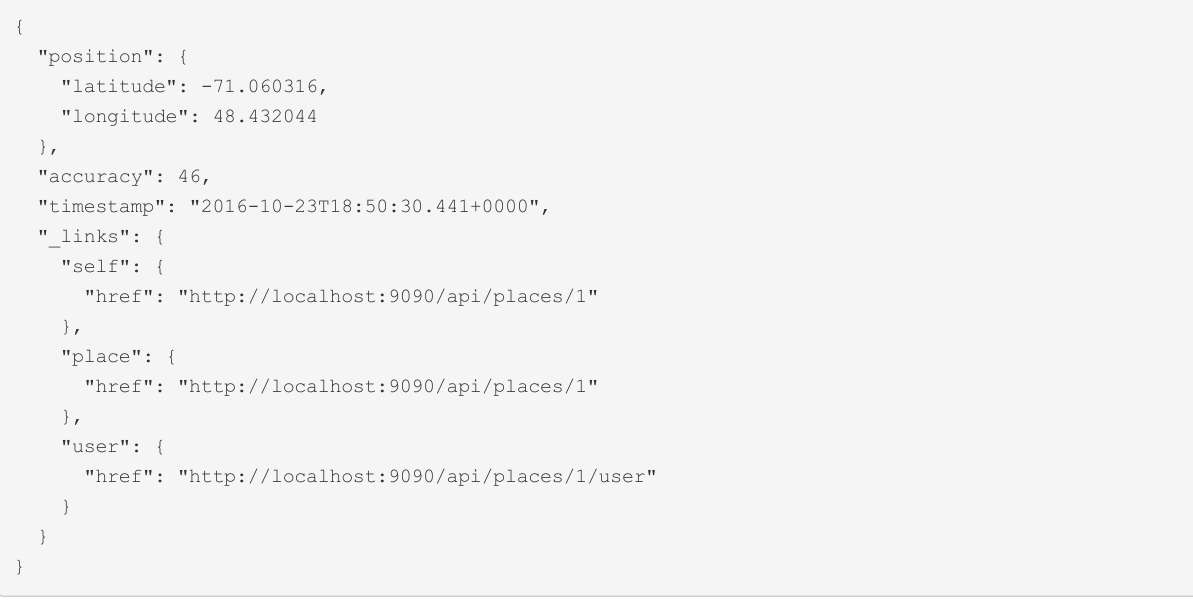
\includegraphics[width=140mm]{images/request.png}
  \caption{Παράδειγμα απάντησης σε JSON μορφή}
  \label{fig:request}
\end{figure}

Για να γίνουν αντιληπτά τα παραπάνω στο διάγραμμα ~\ref{fig:request} εμφανίζεται ένα απλό παράδειγμα απάντησης ενός εξυπηρετητή που χρησιμοποιεί ReST API. Ο πελάτης χρησιμοποιώντας το HTTP πρωτόκολλο έκανε μία αίτηση στο URL:

\textbf{http://servername.com/api/places/1}

ζητώντας να του επιστραφούν οι πληροφορίες της περιοχής με ταυτότητα 1.

\subsection{Websockets}
Όπως αναφέραμε παραπάνω ένα ReST API βασίζεται στην αρχή αίτησης-απάντησης με αποτέλεσμα ο πελάτης να είναι αναγκασμένος να δημιουργεί πολλαπλά αιτήματα. Η μέθοδος αυτή λειτουργεί σε περιπτώσεις που ο πελάτης δεν έχει την ανάγκη να λαμβάνει άμεσα οποιαδήποτε αλλαγή στα δεδομένα τα οποία των απασχολούν 
. Υπάρχουν όμως περιπτώσεις στις οποίες η επικοινωνία μεταξύ πελάτη και εξυπηρετητή πρέπει να είναι αμφίδρομη. Υπάρχουν σενάρια στα οποία ο εξυπηρετητής πρέπει να ενημερώνει τον πελάτη χωρίς την ανάγκη δημιουργίας ενός νέου αιτήματος. Για την επίλυση του παραπάνω προβλήματος μπορεί να γίνει χρήση των websocket.
\par
Το websocket είναι ένα πρωτόκολλο τυποποιημένο από τον οργανισμό IETF \citep{websockets}. Καθιστά δυνατή τη πλήρη αμφίδρομη επικοινωνία μεταξύ πελάτη και εξυπηρετητή στο επίπεδο του TCP. Η αρχική επικοινωνία μεταξύ πελάτη και εξυπηρετητή επιτυγχάνεται μέσω HTTP. Εφόσον η επικοινωνία θεωρηθεί επιτυχείς το πρωτόκολλο αναβαθμίζεται σε websocket. Έτσι δημιουργείται ένας αγωγός μεταξύ πελάτη και εξυπηρετητή ο οποίος μπορεί να χρησιμοποιηθεί και από τους δύο.

\begin{figure}[h]
  \centering
  \includegraphics[width=140mm]{images/websocket.png}
  \caption{Παράδειγμα επικοινωνίας μέσω websocket}
  \label{fig:websocket}
\end{figure}

\newpage

\subsection{Publish-Subscribe}
Publish-subscribe είναι ένα μοτίβο αποστολής μηνυμάτων στο οποίο οι αποστολείς δεν στέλνουν τα μηνύματα τους άμεσα στους αποδέκτες, αλλά αποστέλλονται σε ένα διαμεσολαβητή ο οποίος είναι υπεύθυνος για τη δρομολόγησή τους \citep{publishSubscribeWiki}. Ένα απλό παράδειγμα βιβλιοθήκης η οποία επιτρέπει τη χρήση του μοτίβου publish-subscribe μέσω του websocket πρωτοκόλλου είναι η βιβλιοθήκη Stomp. Ο τρόπος λειτουργίας όπως εμφανίζεται στο διάγραμμα ~\ref{fig:publish-subscribe} είναι ο εξής:

\begin{itemize}
\item Δημιουργείται ένα θέμα το οποίο μπορεί να απασχολεί τους χρήστες (topic).
\item Οι χρήστες οι οποίοι ενδιαφέρονται για το παραπάνω θέμα γίνονται συνδρομητές πάνω σε αυτό (subscribe).
\item Κάποιος από τους χρήστες στέλνει κάποιο μήνυμα στο παραπάνω θέμα (publish).
\item Τέλος οι συνδρομητές που έχουν εγγραφεί στο παραπάνω θέμα λαμβάνουν το μήνυμα που δημοσιεύθηκε.
\end{itemize}


\begin{figure}[h]
  \centering
  \includegraphics[width=120mm]{images/publish-subscribe.png}
  \caption{Παράδειγμα publish-subscribe}
  \label{fig:publish-subscribe}
\end{figure}

\subsection{Spring Framework}
Από τις παραπάνω πληροφορίες είναι φανερή η ανάγκη εύρεσης ενός εργαλείου το οποίο θα βοηθήσει στην ανάπτυξη του web service. Ένα από τα πιο ισχυρά εργαλεία είναι το Spring Framework. Το Spring framework χαρακτηρίζεται ως ένα application framework το οποίο εξυπηρετεί στην δόμηση της εφαρμογής \citep{springframework}. Στο συγκεκριμένο σύστημα χρησιμοποιήθηκε στη δημιουργία ενός σύνθετου εξυπηρετητή ο οποίος θα μπορεί να παρέχει υπηρεσίες στους πελάτες του. Έτσι με τη βοήθεια του Spring framework ήταν δυνατή η δημιουργία ενός εξυπηρετητή που παρέχει ένα ReST API καθώς και τη δυνατότητα publish-subscribe μέσω websockets.

\chapter{Περιγραφή περιπτώσεων χρήσης}

\section{Εισαγωγή}
Σε αυτό το κεφάλαιο θα αναλύσουμε τις περιπτώσεις χρήσης του συστήματος. Θα αποφύγουμε να εισέλθουμε σε λεπτομέρειες του σχεδιασμού και της υλοποίησης του συστήματος καθώς υπάρχει κεφάλαιο παρακάτω αφιερωμένο σε αυτό το σκοπό.

\section{Εφαρμογή κινητών συσκευών}

\subsection{Σενάρια χρήσης}
Ο χρήστης θα πρέπει να μπορεί να χρησιμοποιήσει την εφαρμογή ανεξαρτήτως πλατφόρμας κινητής συσκευής. Παρακάτω θα παρουσιαστούν οι διάφορες περιπτώσεις χρήσης της εφαρμογής σε μορφή πίνακα \citep{uml}.

%--------------------- USE-CASE 1

\begin{table}[h]
 \caption{Δημιουργία νέου λογαριασμού}
\begin{center}
\begin{tabular}{ | m{10em} |  m{25em} | } 
\hline
 Τίτλος & Δημιουργία νέου λογαριασμού \\ 
\hline
 Περιγραφή & Ο χρήστης θα μπορεί να δημιουργήσει ένα προσωπικό λογαριασμό για να μπορέσει να χρησημοποιήσει την εφαρμογή. \\ 
\hline
 Επιτυχές σενάριο &  Ο χρήστης δημιουργεί ένα νέο προσωπικό λογαριασμό.\\
\hline
 Ανεπιτυχές σενάριο  & Ο χρήστης αποτυγχάνει καθώς το usename είναι καταχωρυμένο σε άλλο χρήστη. \\ 
\hline
 Βασικοί χρήστες  & Απλός χρήστης \\ 
\hline
 Βασική ροή  & 
\begin{enumerate}
\item Η εφαρμογή εμφανίζει την φόρμα εγγραφής
\item Ο χρήστης συμπληρώνει τα απαραίτητα πεδία
\item Ο χρήστης αποστέλλει τα πεδία
\item Το σύστημα ελέγχει τη ορθότητα των δεδομένων και δημιουργεί το νέο λογαριασμό χρήστη
\end{enumerate}
 \\ 
\hline
 Εναλλακτικό σενάριο  & Αποτυχία δημιουργίας λογαριασμού  \\ 
\hline
\end{tabular}
\end{center}
\end{table}

%--------------------- USE-CASE 2

\begin{table}[h]
 \caption{Είσοδος του χρήστη στην εφαρμογή}
\begin{center}
\begin{tabular}{ | m{10em} |  m{25em} | } 
\hline
 Τίτλος & Είσοδος του χρήστη στην εφαρμογή \\ 
\hline
 Περιγραφή & Ο χρήστης θα μπορεί να εισέρχεται στην εφαρμογή κάνοντας χρήση του username και password. \\ 
\hline
 Επιτυχές σενάριο & Ο χρήστης εισέρχεται με επιτυχία στην εφαρμογή.\\
\hline
 Ανεπιτυχές σενάριο  & Ο χρήστης  αποτυγχάνει καθώς τα διαπιστευτήριά του είναι λανθασμένα. \\ 
\hline
 Βασικοί χρήστες  & Απλός χρήστης \\ 
\hline
 Βασική ροή  & 
\begin{enumerate}
\item Η εφαρμογή εμφανίζει την φόρμα εισόδου
\item Ο χρήστης συμπληρώνει τα απαραίτητα πεδία
\item Ο χρήστης αποστέλλει τα πεδία
\item Το σύστημα ελέγχει τη ορθότητα των δεδομένων και επιτρέπει την είσοδο του χρήστη
\end{enumerate}
 \\ 
\hline
 Εναλλακτικό σενάριο  & Αποτυχία εισόδου του χρήστη  \\ 
\hline
\end{tabular}
\end{center}
\end{table}

%--------------------- USE-CASE 3

\begin{table}[h]
 \caption{Ενεργοποίηση της καταγραφής των τοποθεσιών του χρήστη.}
\begin{center}
\begin{tabular}{ | m{10em} |  m{25em} | } 
\hline
 Τίτλος & Ενεργοποίηση της καταγραφής των τοποθεσιών του χρήστη. \\ 
\hline
 Περιγραφή & Ο χρήστης θα μπορεί να ενεργοποιήσει την καταγραφή των τοποθεσιών του. \\ 
\hline
 Επιτυχές σενάριο & Ο χρήστης ενεργοποιεί με επιτυχία την καταγραφή.\\
\hline
 Ανεπιτυχές σενάριο  & Η συσκευή αποτυγχάνει να εκκινήσει την υπηρεσία καταγραφής. \\ 
\hline
 Βασικοί χρήστες  & Απλός χρήστης \\ 
\hline
 Βασική ροή  & 
\begin{enumerate}
\item Η εφαρμογή εμφανίζει την σελίδα καταγραφής τοποθεσιών
\item Ο χρήστης ενεργοποιεί την καταγραφή
\item Η υπηρεσία εκκινεί την καταγραφή στο πίσω μέρος της εφαρμογής
\end{enumerate}
 \\ 
\hline
 Εναλλακτικό σενάριο  & Αποτυχία εκκίνησης της υπηρεσίας  \\ 
\hline
\end{tabular}
\end{center}
\end{table}

%--------------------- USE-CASE 4

\begin{table}[h]
 \caption{Εμφάνιση των καταγεγραμμένων τοποθεσιών του χρήστη}
\begin{center}
\begin{tabular}{ | m{10em} |  m{25em} | } 
\hline
 Τίτλος & Εμφάνιση των καταγεγραμμένων τοποθεσιών του χρήστη. \\ 
\hline
 Περιγραφή & Ο χρήστης θα μπορεί να εμφανίζει τις καταγεγραμμένες τοποθεσίες του σε ένα χάρτη. \\ 
\hline
 Επιτυχές σενάριο & Ο χρήστης βλέπει τις τοποθεσίες του να εμφανίζονται στο χάρτη.\\
\hline
 Ανεπιτυχές σενάριο  & Η εφαρμογή αποτυγχάνει να ανακαλέσει τις τοποθεσίες του χρήστη. \\ 
\hline
 Βασικοί χρήστες  & Απλός χρήστης \\ 
\hline
 Βασική ροή  & 
\begin{enumerate}
\item Ο χρήστης επιλέγει την σελίδα εμφάνισης των τοποθεσιών από το μενού επιλογών της εφαρμογής.
\item Η εφαρμογή φορτώνει τις τοποθεσίες του χρήστη.
\item Γίνεται εμφάνιση των τοποθεσιών στο χάρτη
\end{enumerate}
 \\ 
\hline
 Εναλλακτικό σενάριο  & Αποτυχία εύρεσης τοποθεσιών και εμφάνιση άδειου χάρτη \\ 
\hline
\end{tabular}
\end{center}
\end{table}



\begin{table}[h]
 \caption{Αποστολή προειδοποίησης από το χρήστη σε άλλους χρήστες.}
\begin{center}
\begin{tabular}{ | m{10em} |  m{25em} | } 
\hline
 Τίτλος & Αποστολή προειδοποίησης από το χρήστη σε άλλους χρήστες. \\ 
\hline
 Περιγραφή & Ο χρήστης θα έχει τη δυνατότητα αποστολής προειδοποιήσεων σε άλλους χρήστες σε περίπτωση που είναι φορέας κάποιας ασθένειας. \\ 
\hline
 Επιτυχές σενάριο & Ο χρήστης αποστέλλει με επιτυχία προειδοποίηση στους άλλους χρήστες.\\
\hline
 Ανεπιτυχές σενάριο  & Η εφαρμογή αποτυγχάνει να αποστείλει την προειδοποίηση του χρήστη. \\ 
\hline
 Βασικοί χρήστες  & Απλός χρήστης \\ 
\hline
 Βασική ροή  & 
\begin{enumerate}
\item Ο χρήστης επιλέγει την σελίδα προειδοποιήσεων από το μενού επιλογών της εφαρμογής.
\item Ο χρήστης κάνει κλικ στο κουμπί δημιουργίας νέας προειδοποίησης.
\item Η συσκεύη στέλνει στον εξυπηρετητή την προειδοποίηση του χρήστη.
\end{enumerate}
 \\ 
\hline
 Εναλλακτικό σενάριο  & Αποτυχία αποστολής της προειδοποίησης στον εξυπηρετητή.\\ 
\hline
\end{tabular}
\end{center}
\end{table}

%--------------------- USE-CASE 6

\begin{table}[h]
 \caption{Ειδοποίηση του χρήστη σε περίπτωση επαφής με κάποιο χρήστη φορέα.}
\begin{center}
\begin{tabular}{ | m{10em} |  m{25em} | } 
\hline
 Τίτλος & Ειδοποίηση του χρήστη σε περίπτωση επαφής με κάποιο χρήστη φορέα. \\ 
\hline
 Περιγραφή & Ο χρήστης θα έχει τη δυνατότητα ενεργοποίησης της υπηρεσίας παρακολούθησης ειδοποιήσεων από άλλους χρήστες φορείς κάποιας ασθένειας. \\ 
\hline
 Επιτυχές σενάριο & Ο χρήστης θα ενεργοποιεί με επιτυχία την υπηρεσία παρακολούθησης ειδοποιήσεων από άλλους χρήστες.\\
\hline
 Ανεπιτυχές σενάριο  & Η εφαρμογή αποτυγχάνει να εκκινήσει την υπηρεσία. \\ 
\hline
 Βασικοί χρήστες  & Απλός χρήστης \\ 
\hline
 Βασική ροή  & 
\begin{enumerate}
\item Ο χρήστης επιλέγει την σελίδα προειδοποιήσεων από το μενού επιλογών της εφαρμογής.
\item Ο χρήστης  θα μπορεί να ενεργοποιήσει την υπηρεσία παρακολούθησης ειδοποιήσεων από τις υπηρεσίες υγείας.
\item Η συσκεύη συνδέετε με τον εξυπηρετητή και αναμένει ειδοποιήσεις.
\end{enumerate}
 \\ 
\hline
 Εναλλακτικό σενάριο  & Αποτυχία σύνδεσης με τον εξυπηρετητή.\\ 
\hline
\end{tabular}
\end{center}
\end{table}

\clearpage
\section{Διαδικτυακή εφαρμογή}

\subsection{Σενάρια χρήσης}
Οι υπηρεσίες υγείας θα πρέπει να έχουν πρόσβαση μέσω μιας άλλης διεπαφής χρήστη στις προειδοποιήσει που έχουν αποσταλεί από τους χρήστες. Παρακάτω θα παρουσιαστούν οι διάφορες περιπτώσεις χρήσης της εφαρμογής σε μορφή πίνακα.


%--------------------- USE-CASE 1

\begin{table}[h]
 \caption{Είσοδος των υπηρεσιών υγείας στη εφαρμογή}
\begin{center}
\begin{tabular}{ | m{10em} |  m{25em} | } 
\hline
 Τίτλος & Είσοδος των υπηρεσιών υγείας στη εφαρμογή \\ 
\hline
 Περιγραφή & Οι υπηρεσίες υγείας θα μπορούν να εισέρχονται στην εφαρμογή κάνοντας χρήση προκαθορισμένου όνομα χρήστη και κωδικού.\\ 
\hline
 Επιτυχές σενάριο & Οι υπηρεσίες υγείας εισέρχονται με επιτυχία στην εφαρμογή.\\
\hline
 Ανεπιτυχές σενάριο  & Οι υπηρεσίες υγείας αποτυγχάνουν καθώς τα διαπιστευτήριά τους είναι λανθασμένα. \\ 
\hline
 Βασικοί χρήστες  & Υπηρεσίες υγείας \\ 
\hline
 Βασική ροή  & 
\begin{enumerate}
\item Η εφαρμογή εμφανίζει την φόρμα εισόδου
\item Οι υπηρεσίες υγείας συμπληρώνουν τα απαραίτητα πεδία
\item Οι υπηρεσίες υγείας αποστέλλουν τα πεδία
\item Το σύστημα ελέγχει τη ορθότητα των δεδομένων και επιτρέπει την είσοδο των υπηρεσιών υγείας
\end{enumerate}
 \\ 
\hline
 Εναλλακτικό σενάριο  & Αποτυχία εισόδου στην εφαρμογή \\ 
\hline
\end{tabular}
\end{center}
\end{table}

%--------------------- USE-CASE 2

\begin{table}[h]
 \caption{Εμφάνιση απεσταλμένων ειδοποιήσεων από τους χρήστες}
\begin{center}
\begin{tabular}{ | m{10em} |  m{25em} | } 
\hline
 Τίτλος & Εμφάνιση απεσταλμένων ειδοποιήσεων από τους χρήστες \\ 
\hline
 Περιγραφή & Οι υπηρεσίες υγείας θα μπορούν να παρακολουθούν σε πραγματικό χρόνο τις απεσταλμένες ειδοποιήσεις χρηστών.\\ 
\hline
 Επιτυχές σενάριο & Οι υπηρεσίες υγείας ενεργοποιούν την υπηρεσία παρακολούθησης ειδοποιήσεων των χρηστών.\\
\hline
 Ανεπιτυχές σενάριο  & Η εφαρμογή αποτυγχάνει να εκκινήσει την υπηρεσία. \\ 
\hline
 Βασικοί χρήστες  & Υπηρεσίες υγείας \\ 
\hline
 Βασική ροή  & 
\begin{enumerate}
\item Οι υπηρεσίες υγείας επιλέγουν την σελίδα ειδοποιήσεων από το μενού επιλογών της εφαρμογής.
\item Η συσκεύη συνδέετε με τον εξυπηρετητή και αναμένει ειδοποιήσεις.
\end{enumerate}
 \\ 
\hline
 Εναλλακτικό σενάριο  & Αποτυχία σύνδεσης με τον εξυπηρετητή \\ 
\hline
\end{tabular}
\end{center}
\end{table}

%--------------------- USE-CASE 3

\begin{table}[h]
 \caption{Αποδοχή ή μη μίας απεσταλμένης ειδοποίησης από έναν χρήστη}
\begin{center}
\begin{tabular}{ | m{10em} |  m{25em} | } 
\hline
 Τίτλος & Αποδοχή ή μη μίας απεσταλμένης ειδοποίησης από έναν χρήστη \\ 
\hline
 Περιγραφή & Οι υπηρεσίες υγείας θα μπορούν να μελετήσουν μια απεσταλμένη ειδοποίηση από κάποιον χρήστη και να την αποδεχτούν ή όχι.\\
\hline
 Επιτυχές σενάριο & Οι υπηρεσίες αποδέχονται ή μη με επιτυχία μια απεσταλμένη ειδοποίηση.\\
\hline
 Ανεπιτυχές σενάριο  & Η εφαρμογή αποτυγχάνει να αποστείλει την επιλογή των υπηρεσιών υγείας στον εξυπηρετητή. \\ 
\hline
 Βασικοί χρήστες  & Υπηρεσίες υγείας \\ 
\hline
 Βασική ροή  & 
\begin{enumerate}
\item Οι υπηρεσίες υγείας επιλέγουν μια ειδοποίηση από τη σελίδα ειδοποιήσεων
\item Η εφαρμογή εμφανίζει τις πληροφορίες του χρήστη και της ειδοποίησης
\item Οι υπηρεσίες υγείας διαλέγουν αν αποδέχονται ή όχι την ειδοποίηση κάνοντας κλικ στο αντίστοιχο κουμπί.
\end{enumerate}
 \\ 
\hline
 Εναλλακτικό σενάριο  & Αποτυχία σύνδεσης με τον εξυπηρετητή. \\ 
\hline
\end{tabular}
\end{center}
\end{table}


\chapter{Περιγραφή Συστήματος}

\section{Εισαγωγή}
Βασικός στόχος αυτού του κεφαλαίου είναι να παρουσιάσει αναλυτικά τις μεθόδους με τις οποίες υλοποιήθηκε το σύστημα. Το σύστημα αποτελείται από 3 κύρια επίπεδα υλοποίησης. Το ανώτερο επίπεδο είναι η διεπαφή των χρηστών ή αλλιώς το γραφικό περιβάλλον το οποίο χωρίζεται σε 2 μέρη. Πρώτο είναι η εφαρμογή κινητών συσκευών και δεύτερο η διαδικτυακή εφαρμογή για τις υπηρεσίες υγείας. Στο αμέσως επόμενο επίπεδο είναι ο εξυπηρετητής ο οποίος περιέχει την υλοποίηση του μοντέλου καθώς και το business logic της εφαρμογής. Τέλος στο κατώτερο επίπεδο βρίσκεται η βάση δεδομένων η οποία είναι υπεύθυνη για την αποθήκευση των δεδομένων ολόκληρου του συστήματος.

\begin{figure}[h]
  \centering
  \includegraphics[width=110mm]{images/system.png}
  \caption{Επισκόπηση συστήματος πτυχιακής}
  \label{fig:system}
\end{figure}

\section{Γραφικό περιβάλλον}
Για το σχεδιασμό του γραφικού περιβάλλοντος των δύο εφαρμογών μας, δόθηκε ιδιαίτερη βάση στην εμφάνιση ώστε να παρέχει μια φιλική αίσθηση στο χρήστη κατά τη διάρκεια λειτουργίας της εφαρμογής. Για το σχεδιασμό του περιβάλλοντος ακολουθήσαμε μια απλοϊκή προσέγγιση με βασική αρχή την παραμονή του γραφικού περιβάλλοντος καθαρού χωρίς μεγάλο αριθμό ενεργειών σε κάθε παράθυρο. Παρακάτω θα γίνει ανάλυση των εργαλείων που χρησιμοποιήθηκαν για να επιτευχθούν οι παραπάνω στόχοι. 

\subsection{Εφαρμογή κινητών συσκευών}
Η εφαρμογή υλοποιήθηκε με τη χρήση του Ionic framework. Το Ionic framework προσφέρει έναν αριθμό εξαρτημάτων για τη διευκόλυνση της δημιουργίας του γραφικού περιβάλλοντος σε κινητές συσκευές. Η χρήση των εξαρτημάτων γίνεται με τη χρήση HTML και CSS. Το Ionic framework ύστερα φροντίζει ώστε το αποτέλεσμα να είναι φιλικό απέναντι στις διαφορετικές πλατφόρμες συσκευών. Στο διάγραμμα ~\ref{fig:ionic-modules} παρουσιάζεται μια σειρά από διαφορετικά παράθυρα μιας εφαρμογής για να γίνει κατανοητό πως εμφανίζεται ένα γραφικό περιβάλλον το οποίο έχει παραχθεί με τη χρήση των Ionic εξαρτημάτων.

\begin{figure}[h]
  \centering
  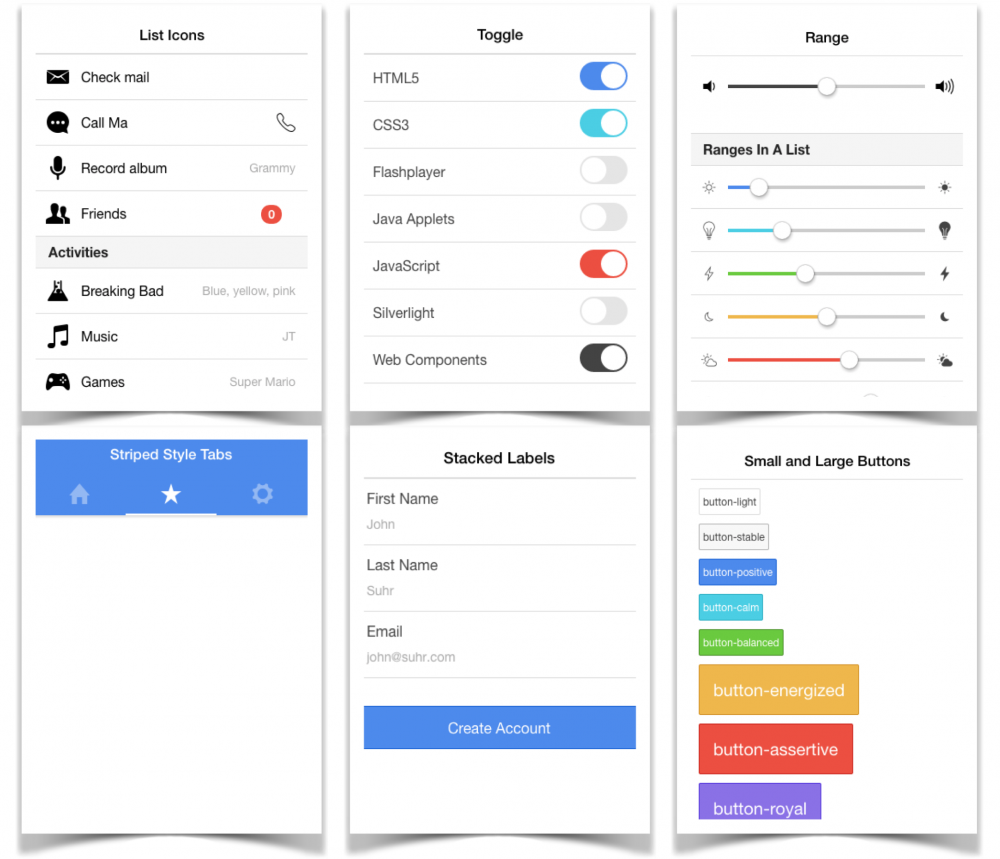
\includegraphics[width=100mm]{images/ionic.png}
  \caption{Επισκόπηση Ιonic εξαρτημάτων}
  \label{fig:ionic-modules}
\end{figure}

\newpage

\subsection{Διαδυκτιακή εφαρμογή}
Βασική προτεραιότητα κατά τη διάρκεια της υλοποίησης της διαδικτυακής εφαρμογής ήταν η παραγωγή μιας εφαρμογής που θα προσφέρει στους χρήστες της ένα μοντέρνο φιλικό περιβάλλον. Για να επιτευχθεί ο παραπάνω στόχος έγινε χρήση του AngularJS framework. Το AngularJS framework προσφέρει τη δυνατότητα δημιουργίας πολύπλοκων εφαρμογών οι οποίες προσαρμόζονται σε μία σελίδα. Οι εφαρμογές SPA καταφέρνουν να δώσουν στο χρήστη την ίδια αίσθηση λειτουργικότητας με μία εφαρμογή ηλεκτρονικών υπολογιστών. Έτσι ο χρήστης δεν χρειάζεται να περιμένει για τη φόρτωση κάποιας σελίδας καθώς ολόκληρη η εφαρμογή προετοιμάζεται μία φορά στην αρχή.

\section{Web Service}
Ο σχεδιασμός και υλοποίηση του web service είχε ως στόχο την παραγωγή ενός API το οποίο ακολουθεί τα πρότυπα της αρχιτεκτονικής ReST. Επίσης γίνεται χρήση της τεχνολογίας websockets και του μοτίβου publish-subscribe. Το web service μπορεί να χωριστεί σε 4 κομμάτια. Παρακάτω θα γίνει ανάλυση των επιμέρους κομματιών του εξυπηρετητή.  

\subsection{Επίπεδο μοντέλου}
Το επίπεδο μοντέλου είναι υπεύθυνο για της εμφάνιση των δεδομένων μας. Παρέχει τη δυνατότητα επεξεργασίας των οντοτήτων μας καθ' όλης τη διάρκεια της εκτέλεσης του συστήματος. Το μοντέλο βοηθάει στη τυποποίηση των οντοτήτων μας και των σχέσεων μεταξύ τους. Πιο συγκεκριμένα το μοντέλο μας λειτουργεί ως ένας διαμεσολαβητής μεταξύ των δεδομένων που αποθηκεύονται στη βάση και των δεδομένων που εμφανίζονται στο χρήστη. 

\subsection{Επίπεδο δεδομένων}
Το επίπεδο δεδομένων λειτουργεί ως διαμεσολαβητής μεταξύ του web service και της βάσης δεδομένων. Είναι υπεύθυνο για της παραλαβή δεδομένων από τη βάση και την αποστολή τους στο επόμενο επίπεδο και το αντίστροφο. Για τη υλοποίηση αυτού του επιπέδου έγινε η χρήση του repository μοτίβου.

\subsubsection{Repository Pattern}
Το repository έχει τη δυνατότητα να μετατρέπει το μοντέλο του συστήματος μας σε δεδομένα δυνατά να αποθηκευτούν στη βάση δεδομένων. Η εύρεση, δημιουργία, ανανέωση, διαγραφή δεδομένων γίνεται μέσω συγκεκριμένων μεθόδων οι οποίες παρέχονται από το repository. Με άλλα λόγια παρέχει μία αφαιρετική δομή ώστε το επίπεδο της λογικής να μην έρχεται σε άμεση επαφή με τη βάση δεδομένων και να μην ασχολείται με τις διάφορες λειτουργίες αυτής όπως σύνδεση, εντολές, πίνακες δεδομένων κ.τ.λ. 

\subsection{Επίπεδο λογικής}
Το επίπεδο λογικής ή αλλιώς business logic είναι το μέλος του συστήματός μας το οποίο φροντίζει για την εφαρμογή των λογικών κανόνων που θέτουμε στο σύστημα μας. Επίσης καθορίζει τη ροή των εργασιών και ποιους από τους κανόνες πρέπει οι εργασίες αυτές να ακολουθήσουν. Τέλος το επίπεδο της λογικής καθορίζει πως το μοντέλο μας αλληλεπιδρά με τα υπόλοιπα μέλη της εφαρμογής.

\subsection{Επίπεδο παρουσίασης}
Το επίπεδο της παρουσίασης, στο web service, λειτουργεί ως διαμεσολαβητής μεταξύ των εφαρμογών μας και του επιπέδου της λογικής. Παρέχει τα απαραίτητα σημεία εισόδου με τη μορφή του ReST API καθώς και τα topics στο κομμάτι των websockets. Το επίπεδο της παρουσίασης είναι ένα λεπτό στρώμα μεταξύ των πελατών και του επιπέδου λογικής. 

\section{Βάση δεδομένων}
Η βάση δεδομένων είναι μια συλλογή από δεδομένα οργανωμένα σε πίνακες οι οποίοι παρουσιάζουν μια οντότητα ο καθένας. Κάθε σειρά του πίνακα αντιστοιχεί σε ένα αντικείμενο αυτής της οντότητας. Στο σύστημά μας έγινε η χρήση της βάσης δεδομένων PostgreSQL. Η PostgreSQL είναι μία σχεσιακή βάση και στη συγκεκριμένη περίπτωση έγινε η χρήση μονάχα πινάκων. Καθώς όμως κάποια από τα δεδομένα είναι γεωγραφικά αντικείμενα δημιουργήθηκε η ανάγκη εύρεσης ενός τρόπου αποθήκευσης και επεξεργασίας αυτού του είδους δεδομένων.

\subsection{PostGIS}
Η επέκταση PostGIS προσφέρει τη δυνατότητα αποθήκευσης γεωγραφικών δεδομένων σε μια βάση PostgreSQL. Προσφέρει μια μεγάλη γκάμα λειτουργιών όπως εύρεση αποστάσεων μεταξύ γεωγραφικών σημείων καθώς ακόμη υπολογισμό επιφανειών μεταξύ αυτών \citep{postgis}. Η χρήση της επέκτασης PostGIS στο σύστημα μας έγινε με σκοπό τη δυνατότητα αποθήκευσης γεωγραφικών σημείων παρέχοντας γεωγραφικό πλάτος και μήκος.

\chapter{Υλοποίηση Συστήματος}

\section{Εισαγωγή}
Στο παρακάτω κεφάλαιο θα παρουσιαστεί αναλυτικά το κάθε επίπεδο υλοποίησης που έχουμε αναφέρει παραπάνω καθώς επίσης θα γίνει μια εκτενής παρουσίαση στα τεχνικά κομμάτια τους. Αρχικά θα παρουσιαστεί το επίπεδο του γραφικού περιβάλλοντος δείχνοντας τα σημαντικότερα λειτουργικά μέρη της εφαρμογής κινητών συσκευών και της διαδικτυακής εφαρμογής. Έπειτα θα γίνει τεχνική ανάλυση του επιπέδου του εξυπηρετητή. Θα αναλυθούν σημαντικά κομμάτια όπως ο μηχανισμός publish/subscribe καθώς και το μοντέλο του συστήματος μας. Τέλος θα παρουσιαστεί το επίπεδο της βάσης δεδομένων παρουσιάζοντας τις οντότητες του συστήματος μας.

\section{Ροή της Εφαρμογής Κινητών}
Ο χρήστης τη πρώτη φορά που θα κάνει χρήση της εφαρμογής μας θα πρέπει να δημιουργήσει ένα καινούριο λογαριασμό. 

\subsection{Ανωνυμία Χρηστών}
Καθώς δίνεται μεγάλη βαρύτητα στα προσωπικά στοιχεία του χρήστη, όπως βλέπουμε στο διάγραμμα ~\ref{fig:login-register} τα μόνα απαραίτητα πεδία είναι το όνομα χρήστη και ο κωδικός. Παρόλα αυτά αν ο χρήστης προσθέσει και τα υπόλοιπα στοιχεία φροντίζουμε για την πλήρη κρυπτογράφηση τους στο επίπεδο της εφαρμογής. 

\begin{figure}[h]
  \centering
  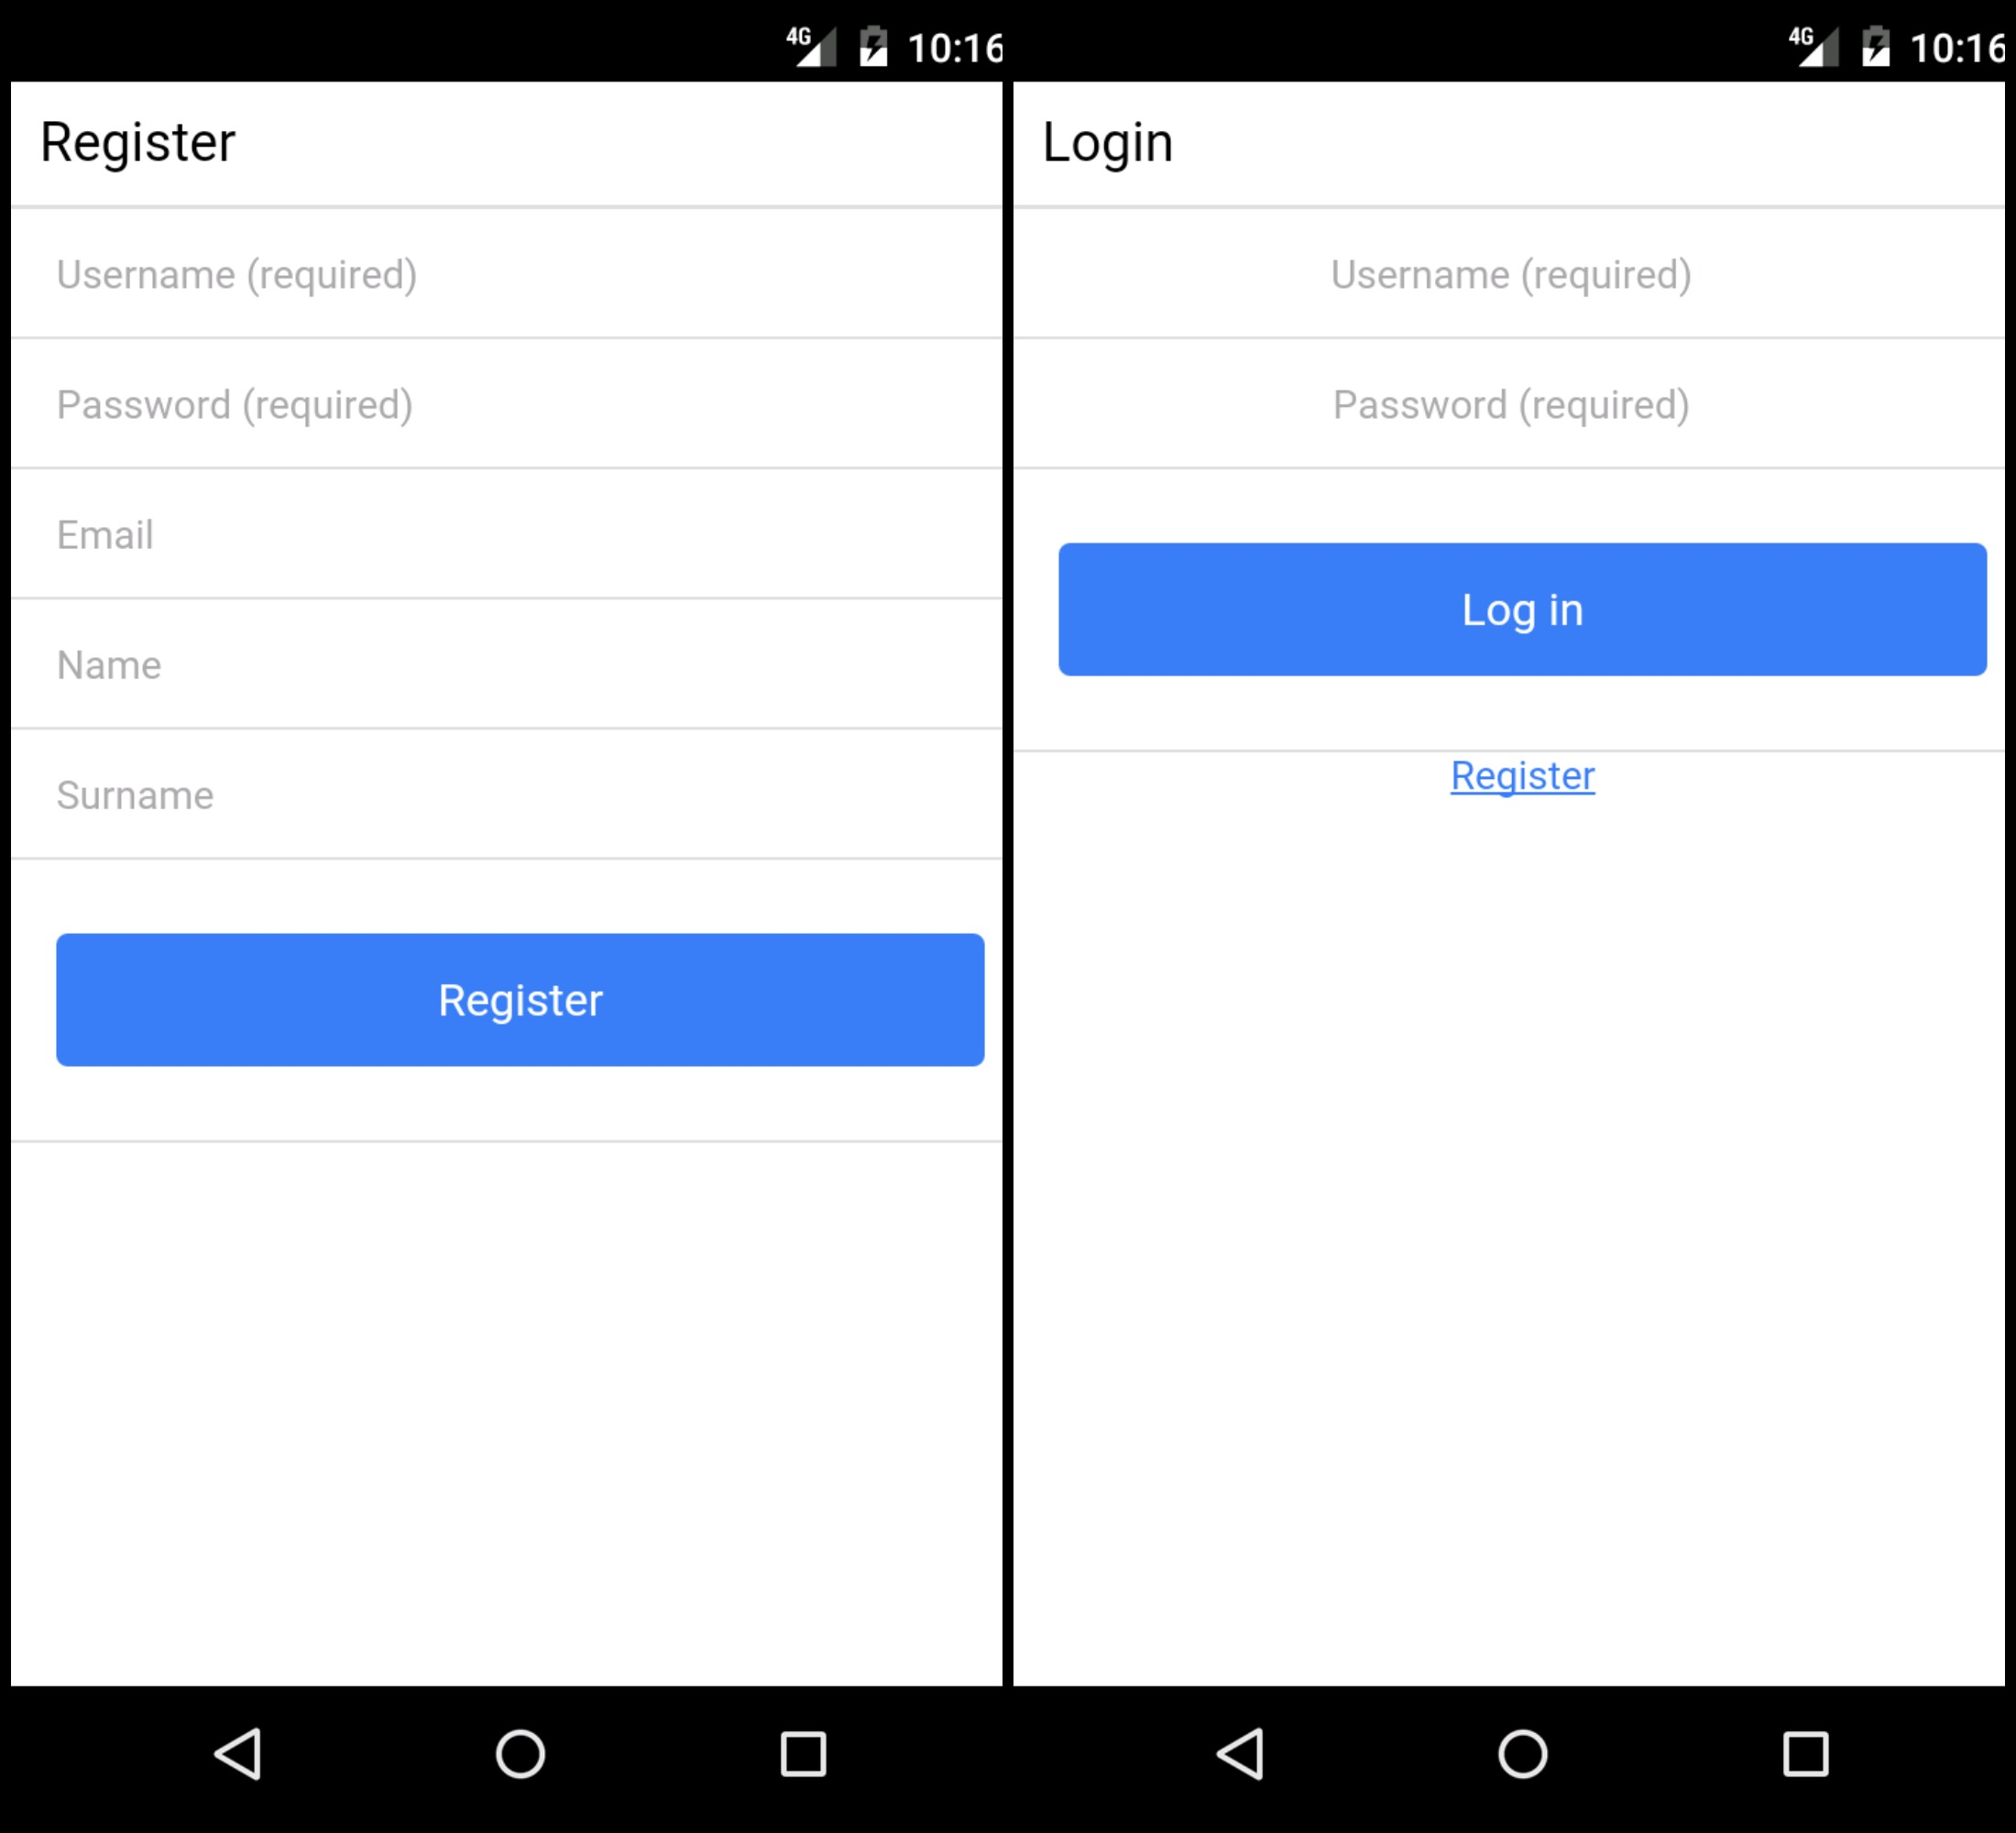
\includegraphics[width=110mm]{images/login-register.jpg}
  \caption{Εγγραφή και σύνδεση}
  \label{fig:login-register}
\end{figure}

\newpage

\subsubsection{CryptoJS}
Η βιβλιοθήκη CryptoJS προσφέρει μια μεγάλη γκάμα αλγόριθμων κρυπτογράφησης σε Javascript. Στη προκειμένη περίπτωση ο αλγόριθμος που χρησιμοποιήσαμε είναι ο AES. Όπως παρατηρούμε στον αλγόριθμο \ref{lst:encryption} πριν την ολοκλήρωση της εγγραφής του χρήστη φροντίζουμε όλα τα στοιχεία του χρήστη να αποσταλούν κρυπτογραφημένα με κλειδί τον κωδικό του. Έτσι επιτυγχάνεται η ανωνυμία του χρήστη καθώς μόνο αυτός έχει τη δυνατότητα να αποκρυπτογραφήσει και να εμφανίσει τα στοιχεία του.

\begin{lstlisting}[language=Java, caption=Κρυπτογράφηση Στοιχείων, label={lst:encryption}]

 $scope.doRegister = function () {
    $scope.encryptUserInformation();
    LoginService.register($scope.registerInfo).then(function (response) {
      $scope.closeRegister();
    });

  };

 $scope.encryptUserInformation = function () {
    $scope.registerInfo.email = $scope.encryptValue($scope.registerInfo.email);
    $scope.registerInfo.name = $scope.encryptValue($scope.registerInfo.name);
    $scope.registerInfo.surname = $scope.encryptValue($scope.registerInfo.surname);
  }

  $scope.encryptValue = function (value) {
    var text = CryptoJS.AES.encrypt(value, $scope.registerInfo.password);
    return text.toString();
  }
\end{lstlisting}

\subsection{Παρακολούθηση τοποθεσιών}
Μετά την εγγραφή και σύνδεση του, ο χρήστης βλέπει στην αρχική σελίδα, όπως παρουσιάζεται στο διάγραμμα ~\ref{fig:watch-position}, στην οποία έχει τη δυνατότητα εκκίνησης παρακολούθησης των τοποθεσιών του.

\begin{figure}[h]
  \centering
  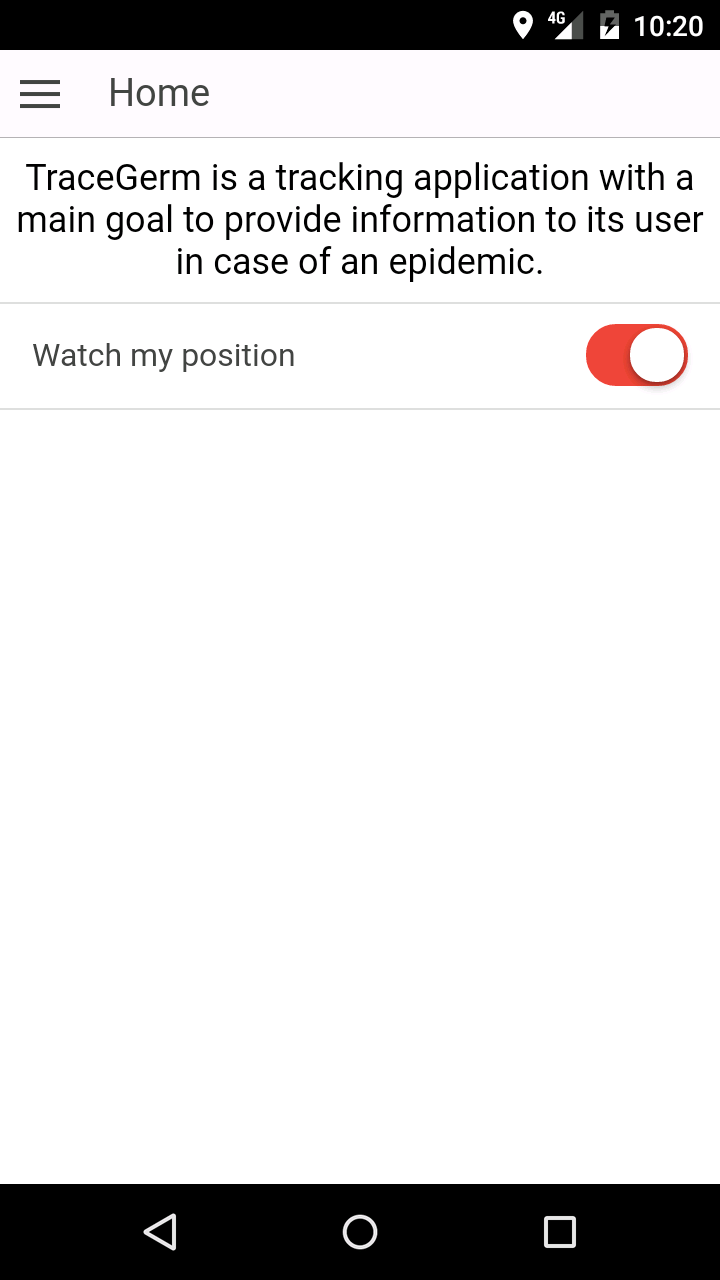
\includegraphics[width=60mm]{images/watch-position.png}
  \caption{Αρχική σελίδα εφαρμογής}
  \label{fig:watch-position}
\end{figure}

\newpage

Μετά την επιλογή του χρήστη να εκκινήσει τη παρακολούθηση, η εφαρμογή εκτελεί τον κώδικα που εμφανίζεται στον αλγόριθμο ~\ref{lst:watch-position}. Κάνοντας χρήση των δυνατοτήτων του Cordova framework λαμβάνουμε τις τοποθεσίες του χρήστη και τις αποστέλλουμε στον εξυπηρετητή για επεξεργασία και αποθήκευση.

\begin{lstlisting}[language=Java, caption=Παρακολούθηση τοποθεσιών, label={lst:watch-position}]
watchPosition: function () {
      watch = $cordovaGeolocation.watchPosition(watchOptions);
      watch.then(
        null,
        function (err) {
          console.log(JSON.stringify(err));
        },
        function (rawPosition) {
          var position = {
            position: {
              latitude: rawPosition.coords.latitude,
              longitude: rawPosition.coords.longitude
            },
            accuracy: rawPosition.coords.accuracy,
            timestamp: rawPosition.timestamp
          };
          HttpSecure.post(apiUrl + '/places', position).success(function (response) {
            console.log(JSON.stringify(response));
          }).catch(function (response) {
            console.log(JSON.stringify(response));
          });
        });
    }
\end{lstlisting}

\subsection{Συναγερμοί Χρήστη}
Πηγαίνοντας στη σελίδα των συναγερμών, ο χρήστης έχει τη δυνατότητα δημιουργίας ενός καινούριου συναγερμού, τον οποίο συναγερμό λαμβάνουν οι υπηρεσίες υγείας και αποδέχονται ή όχι. Επιπλέον δίνεται στο χρήστη η δυνατότητα εγγραφής και παραλαβής ενημερώσεων σε περίπτωση που έχει βρεθεί στην ίδια τοποθεσία με κάποιον άλλο χρήστη του οποίου ο συναγερμός έχει γίνει αποδεκτός από τις υπηρεσίες υγείας. Στο διάγραμμα ~\ref{lst:watch-position} βλέπουμε τις δύο παραπάνω δυνατότητες. 

\begin{figure}[h]
  \centering
  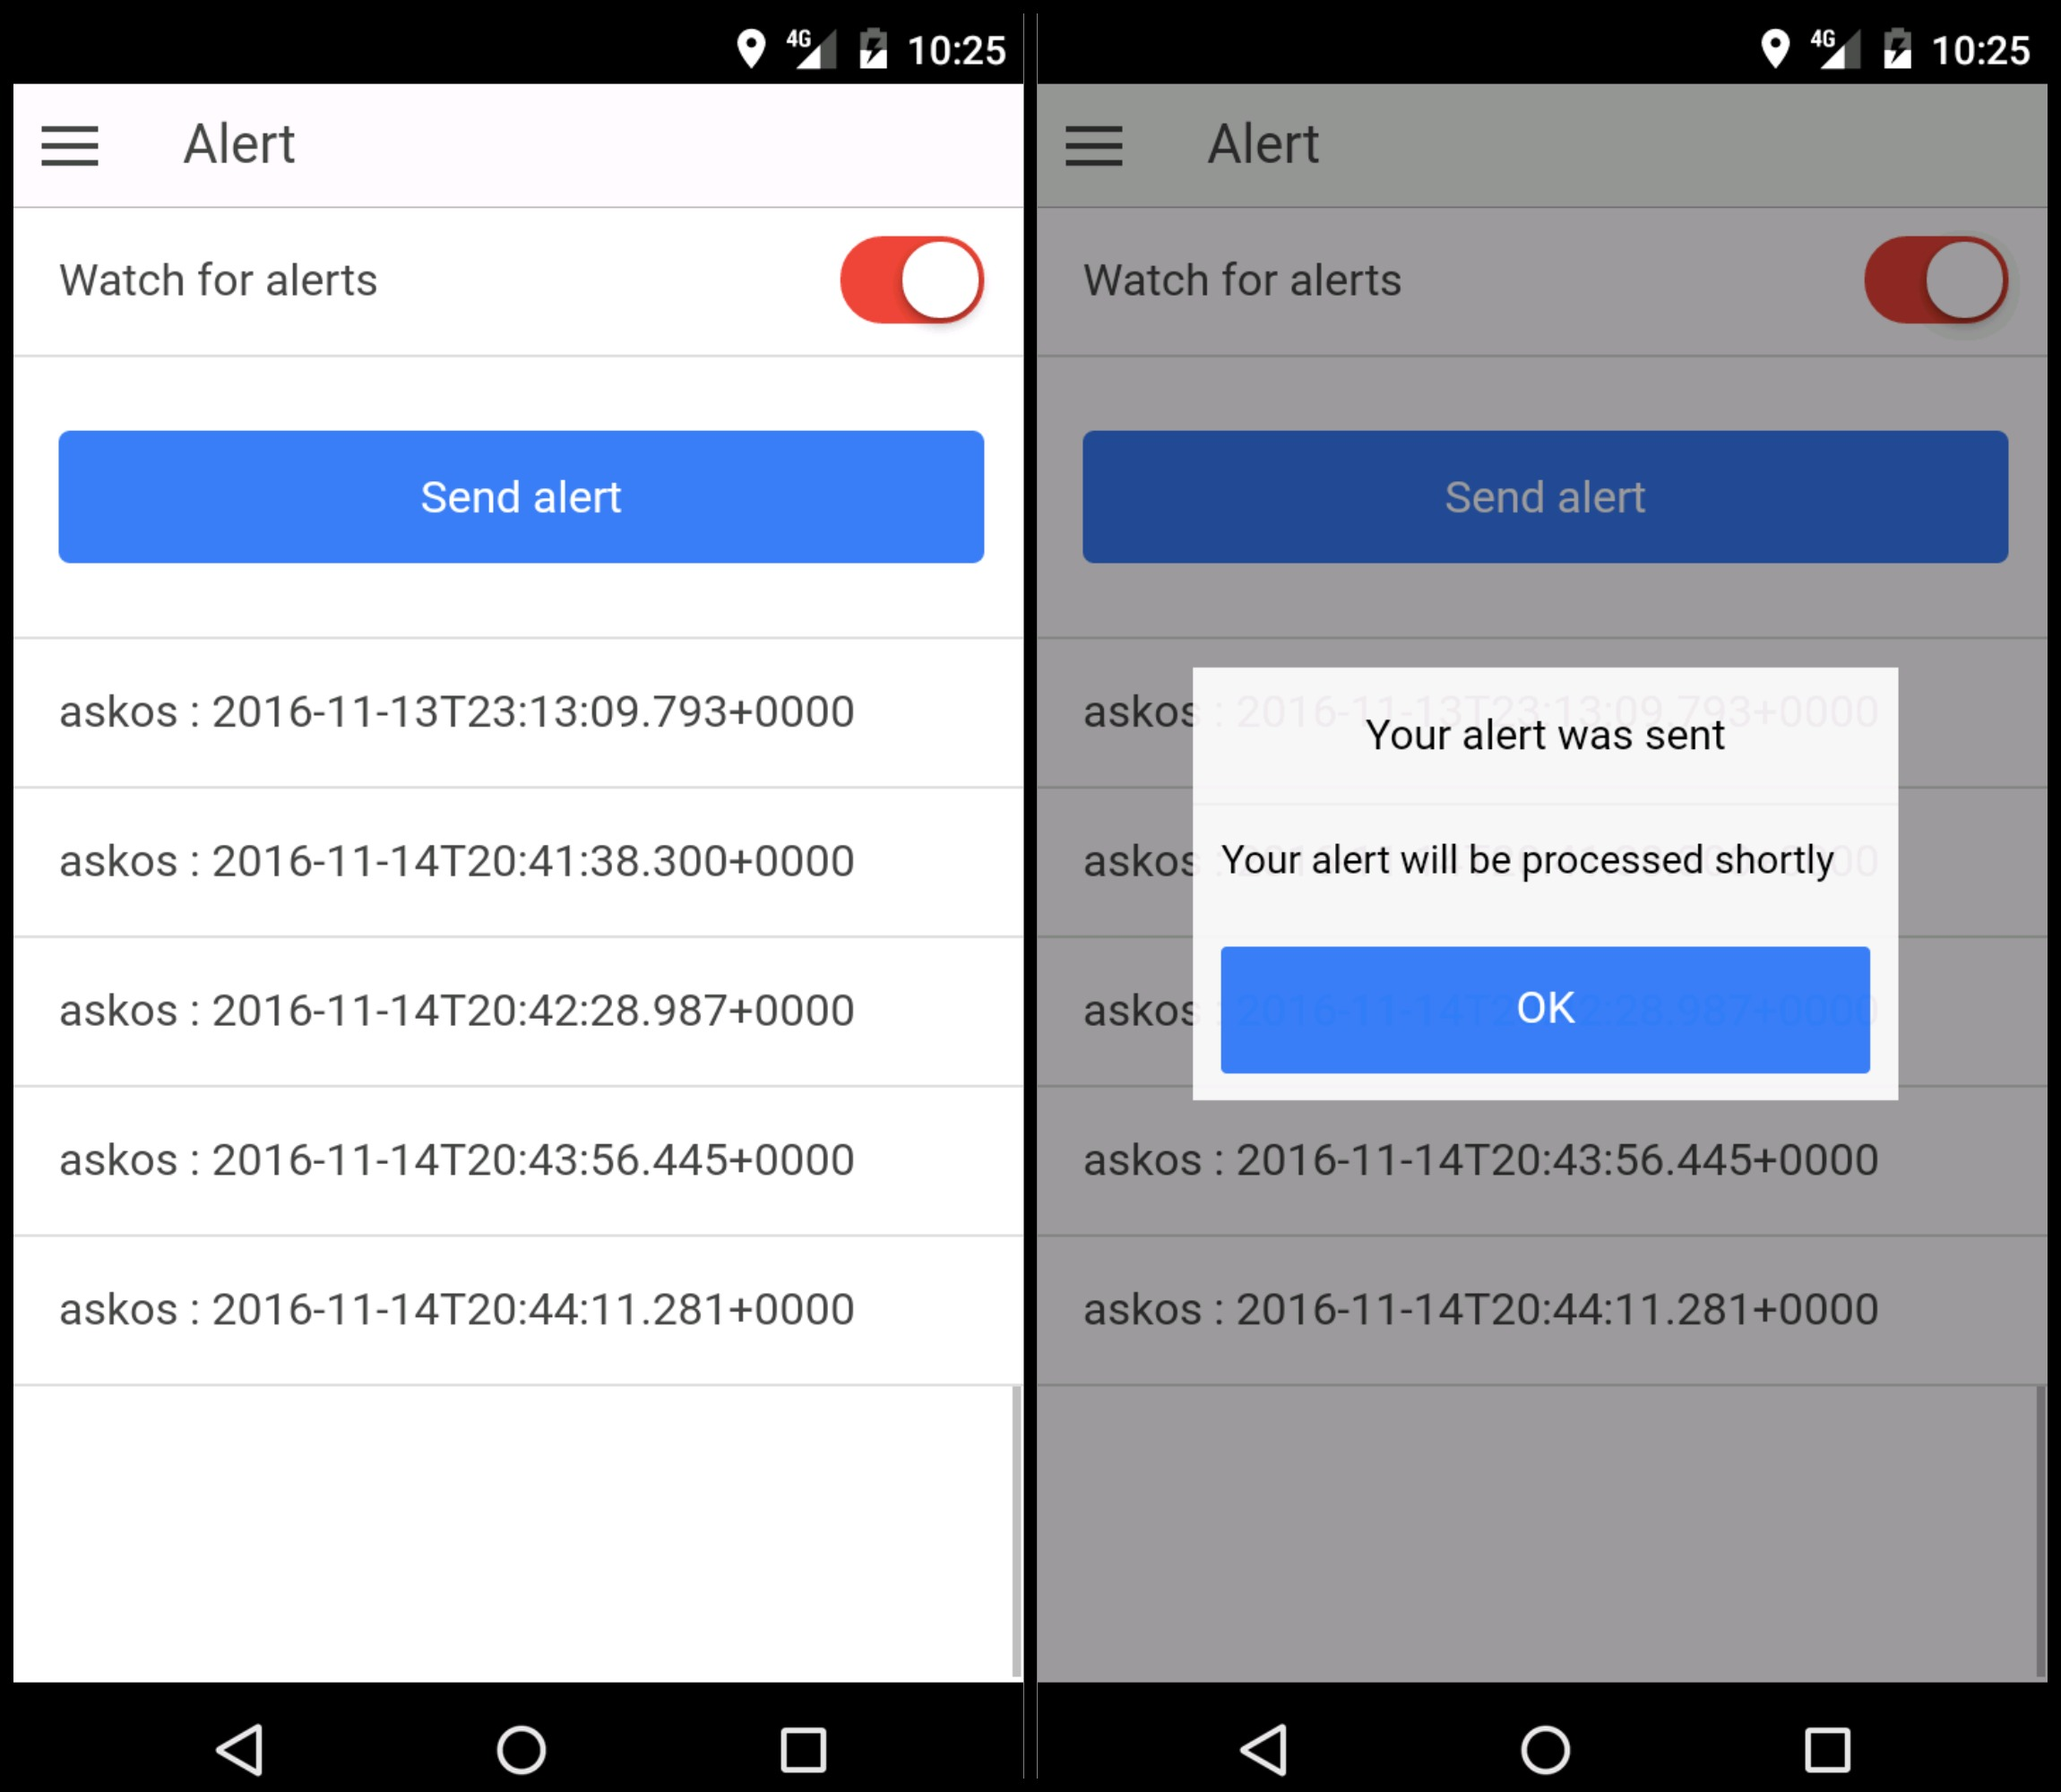
\includegraphics[width=100mm]{images/alerts.jpg}
  \caption{Συναγερμοί}
  \label{fig:alerts}
\end{figure}

\newpage

Ένα σημείο στο οποίο θα πρέπει να δώσουμε βαρύτητα είναι ο τρόπος με τον οποίο ο χρήστης παρακολουθεί για καινούριες ενημερώσεις. Κάνοντας χρήση του μοτίβου publish/subscribe (Αλγόριθμος ~\ref{fig:alerts}) ο χρήστης κάνει έγγραφή στο θέμα των ενημερώσεων οι οποίες τον απασχολούν με αποτέλεσμα να ανοίγεται ένας αγωγός επικοινωνίας με το πρωτόκολλο websocket μεταξύ της συσκευής του χρήστη και του εξυπηρετητή.

\begin{lstlisting}[language=Java, caption=Publish/Subscribe για ενημερώσεις, label={lst:publish_subscribe_notifications}]
$scope.startWatchingAlert = function () {
    $ionicPlatform.ready(function() {
      $scope.socket = new SockJS(apiUrl+'/tracegerm-websocket');
      $scope.stompClient = Stomp.over($scope.socket);
      $scope.stompClient.connect({}, function (frame) {
        $cordovaPreferences.fetch('User')
          .success(function (response) {
            $scope.stompClient.subscribe('/topic/notifications/'+ response.username, function (notification) {
              cordova.plugins.notification.local.schedule({
                title: "Alert!",
                message: "A new notification has appeared"
              });
              $scope.notifications.push(JSON.parse(notification.body));
              $scope.$apply();
            });
          })
      });
    })
  };
\end{lstlisting}

Καθώς αυτός ο αγωγός επικοινωνίας είναι συνεχώς ανοιχτός, ο χρήστης λαμβάνει άμεσα καινούριες ενημερώσεις. Σε αυτό το σημείο είναι σημαντικό να αναφέρουμε ότι για να αποφύγουμε τυχόν χαμένες ειδοποιήσεις οι οποίες δημιουργήθηκαν όταν ο χρήστης για κάποιο λόγο δεν ήταν συνδεδεμένος, φροντίζουμε να φορτώσουμε όλες τις ειδοποιήσεις τις οποίες ο χρήστης δεν έχει αποδεχτεί ακόμη, οι οποίες εμφανίζονται σε μορφή λίστας. Στο διάγραμμα ~\ref{fig:notifications} μπορούμε να παρατηρήσουμε και τις δύο παραπάνω καταστάσεις.   

\begin{figure}[h]
  \centering
  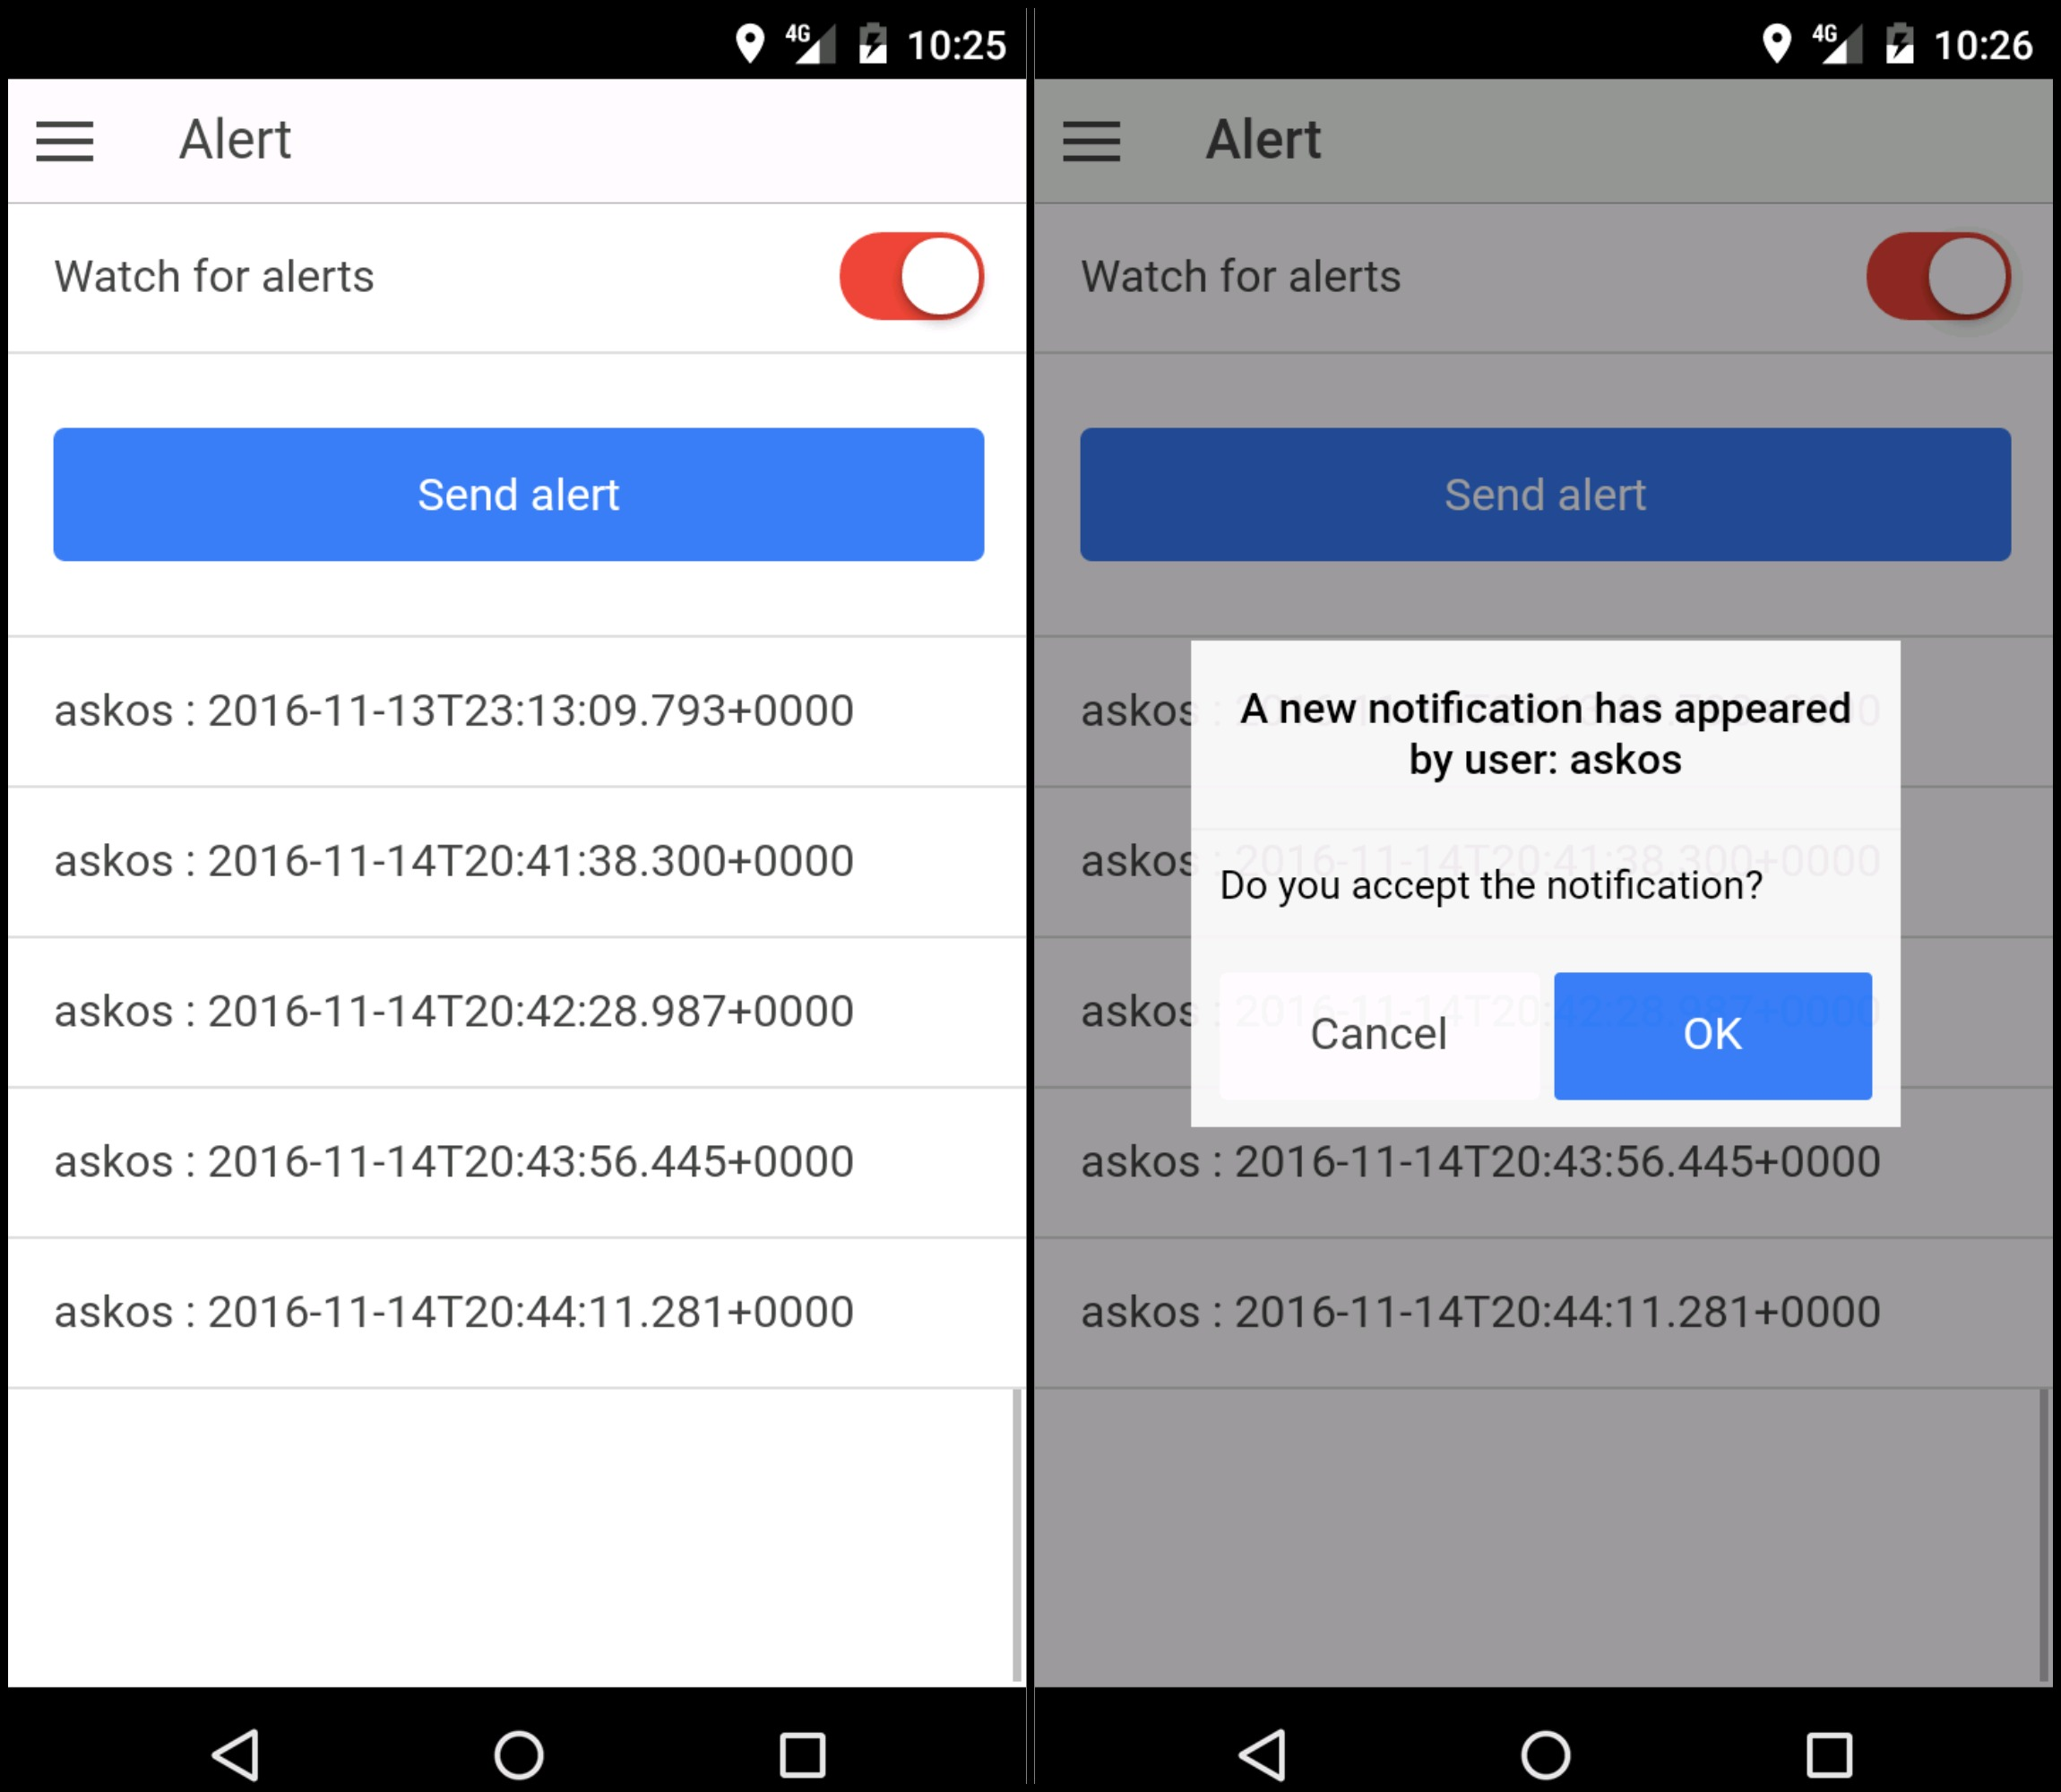
\includegraphics[width=100mm]{images/notifications.jpg}
  \caption{Ενημερώσεις}
  \label{fig:notifications}
\end{figure}

\newpage
\subsection{Τοποθεσίες Χρήστη}
Τέλος, ο χρήστης έχει τη δυνατότητα να δει τις τελευταίες τοποθεσίες τις οποίες επισκέφθηκε μέσω της σελίδας προφίλ. Για να γίνει η εμφάνιση των τοποθεσιών αυτών με ένα φιλικό τρόπο απέναντι στο χρήστης, αποφασίστηκε να γίνει χρήση της υπηρεσίας Google Maps. Έτσι ο χρήστης έχει τη δυνατότητα να δει τις τοποθεσίες του άμεσα σε ένα χάρτη (διάγραμμα ~\ref{fig:locations})  αντί μιας λίστας με γεωγραφικά πλάτη και μήκη.

\begin{figure}[h]
  \centering
  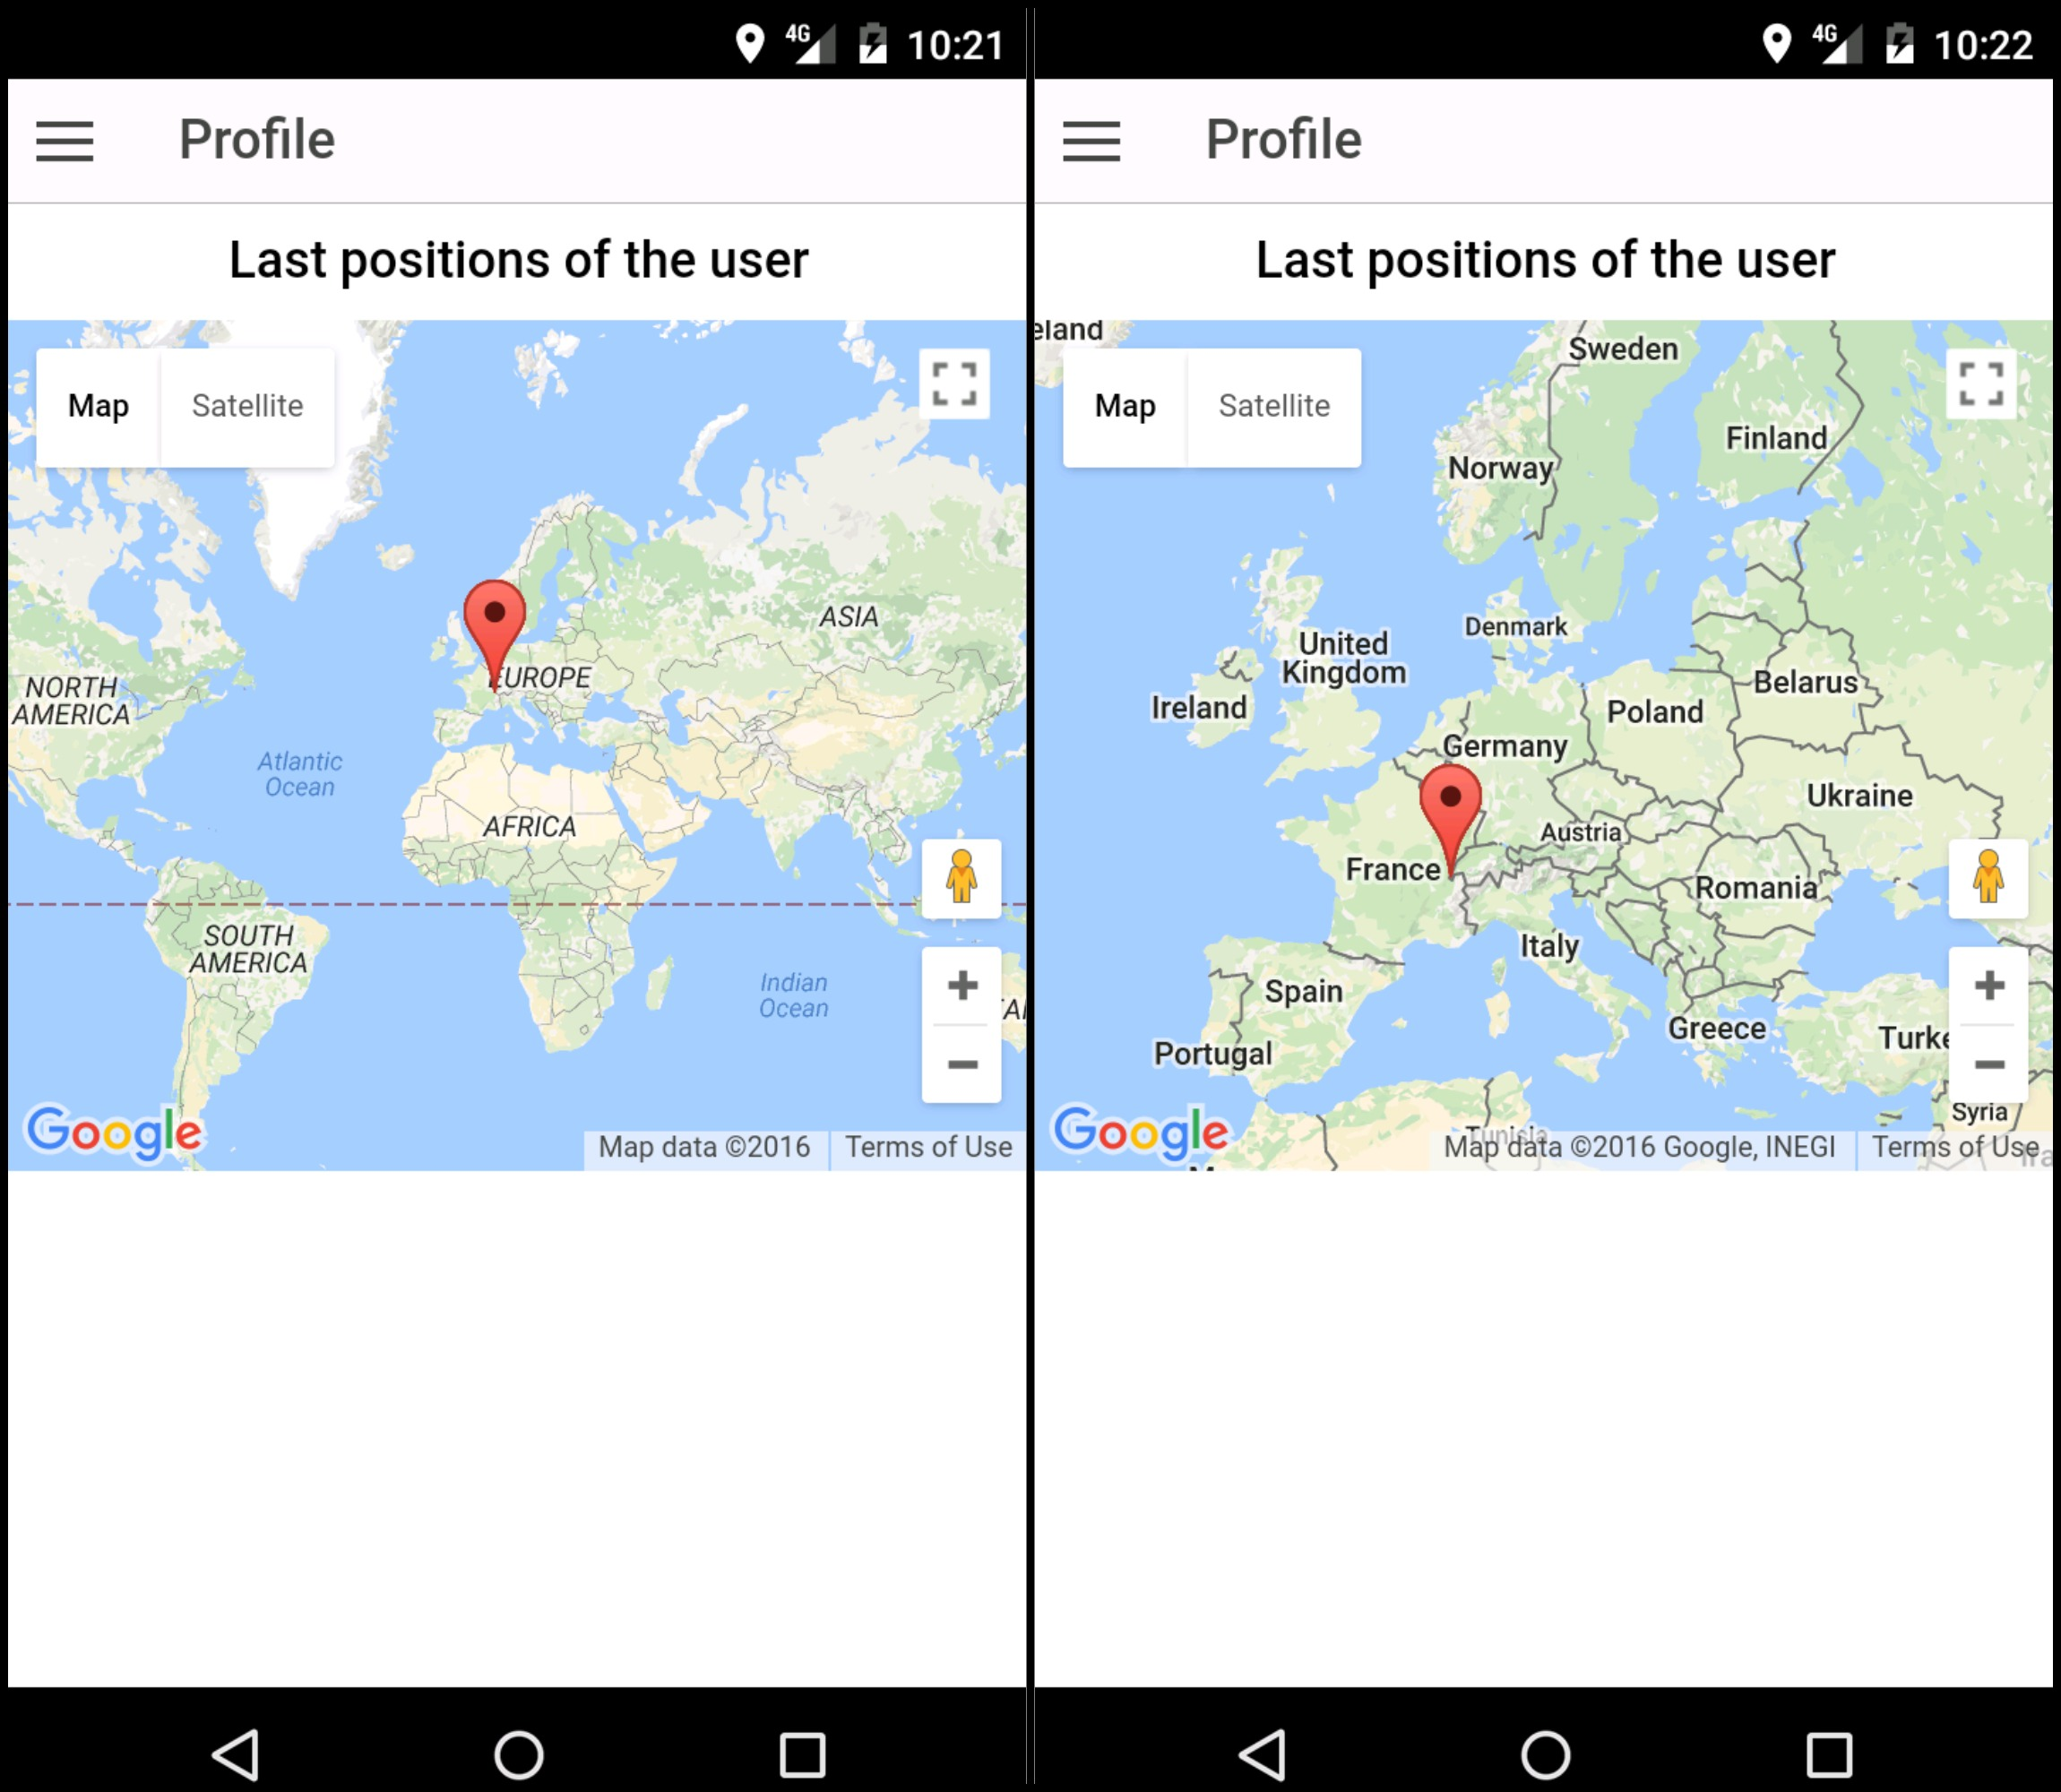
\includegraphics[width=100mm]{images/profile.jpg}
  \caption{Τοποθεσίες χρήστη}
  \label{fig:locations}
\end{figure}

\section{Ροή της Διαδικτυακής Εφαρμογής}
Η διαδικτυακή εφαρμογή είναι σαφώς πιο απλή από την εφαρμογή κινητών συσκευών. Παρακάτω θα παρουσιάσουμε την διεπαφή χρήστη καθώς και τις λειτουργίες της.

\subsection{Είσοδος Υπαλλήλου Υπηρεσιών Υγείας}
Στην αρχική σελίδα της διαδικτυακής εφαρμογής ζητάμε από τους υπαλλήλους των υπηρεσιών υγείας να εισέλθουν κάνοντας χρήση ενός λογαριασμού ο οποίος έχει τον ρόλο διαχειριστή. Με αυτό το τρόπο φροντίζουμε οι χρήστες μας να είναι εξουσιοδοτημένοι και τα στοιχεία των χρηστών μας ασφαλή. Καθώς οι απαραίτητοι έλεγχοι γίνονται στο επίπεδο του εξυπηρετητή, θα αποφύγουμε να μπούμε σε λεπτομέρειες σε αυτό το σημείο και θα αναφερθούμε περαιτέρω αργότερα.

\begin{figure}[h]
  \centering
  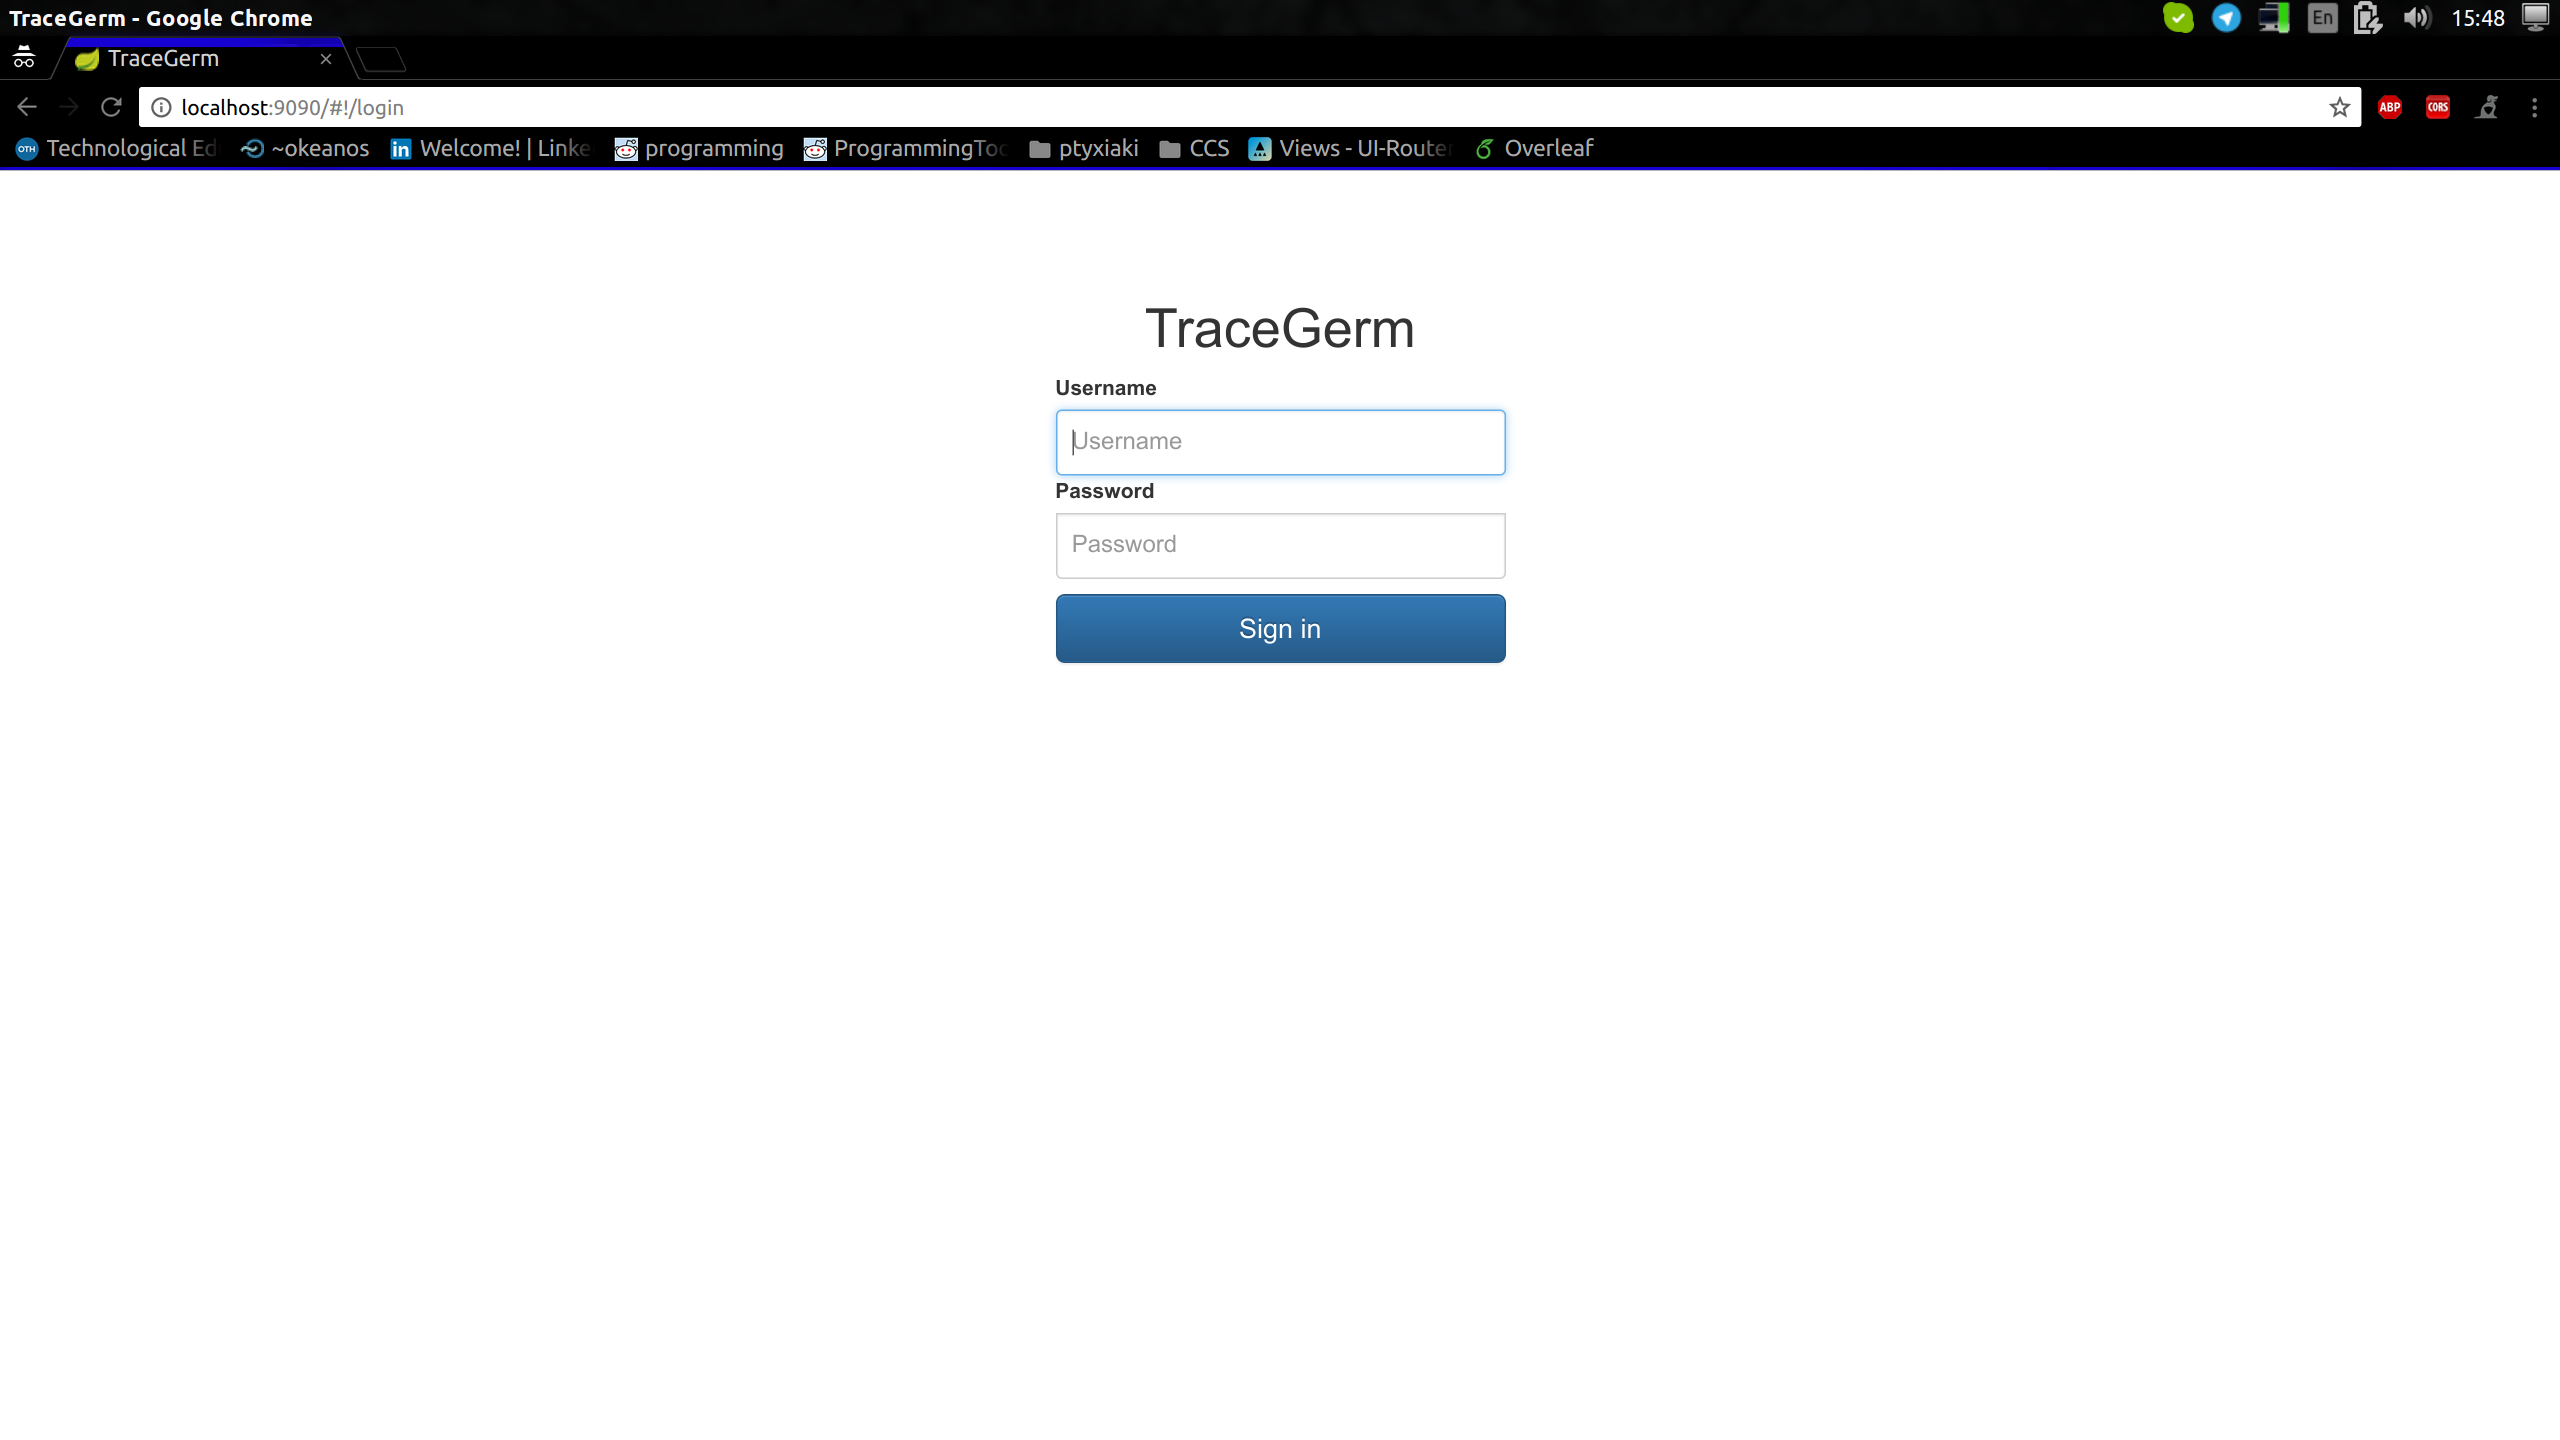
\includegraphics[width=150mm]{images/login.png}
  \caption{Είσοδος Υπαλλήλου Υπηρεσιών Υγείας}
  \label{fig:login-webapp}
\end{figure}

\subsection{Σελίδα συναγερμών}
Καθώς οι υπάλληλοι έχουν εισέλθει στη σελίδα συναγερμών, έχουν τη δυνατότητα να λαμβάνουν σε πραγματικό χρόνο νέους συναγερμούς από τους χρήστες με το πρότυπο publish/subscribe. Κατά συνέπεια οι υπάλληλοι μπορούν να αποδεχτούν ή όχι έναν συναγερμό. Λόγω της κρισιμότητας μιας τέτοιας απόφασης αποφασίστηκε να δοθεί ο πλήρης έλεγχος στους ανθρώπους χωρίς επέμβαση κάποιου αλγόριθμου. Έτσι εάν ένας υπάλληλος αποφασίσει ότι πρέπει να αποδεχτεί τον συναγερμό ενός χρήστη τότε φροντίζουμε να καλέσουμε τον απαραίτητο αλγόριθμο στον εξυπηρετητή για να ενημερώσουμε όλους τους χρήστες οι οποίοι μπορεί να ήρθαν σε επαφή μαζί του.

\begin{figure}[h]
  \centering
  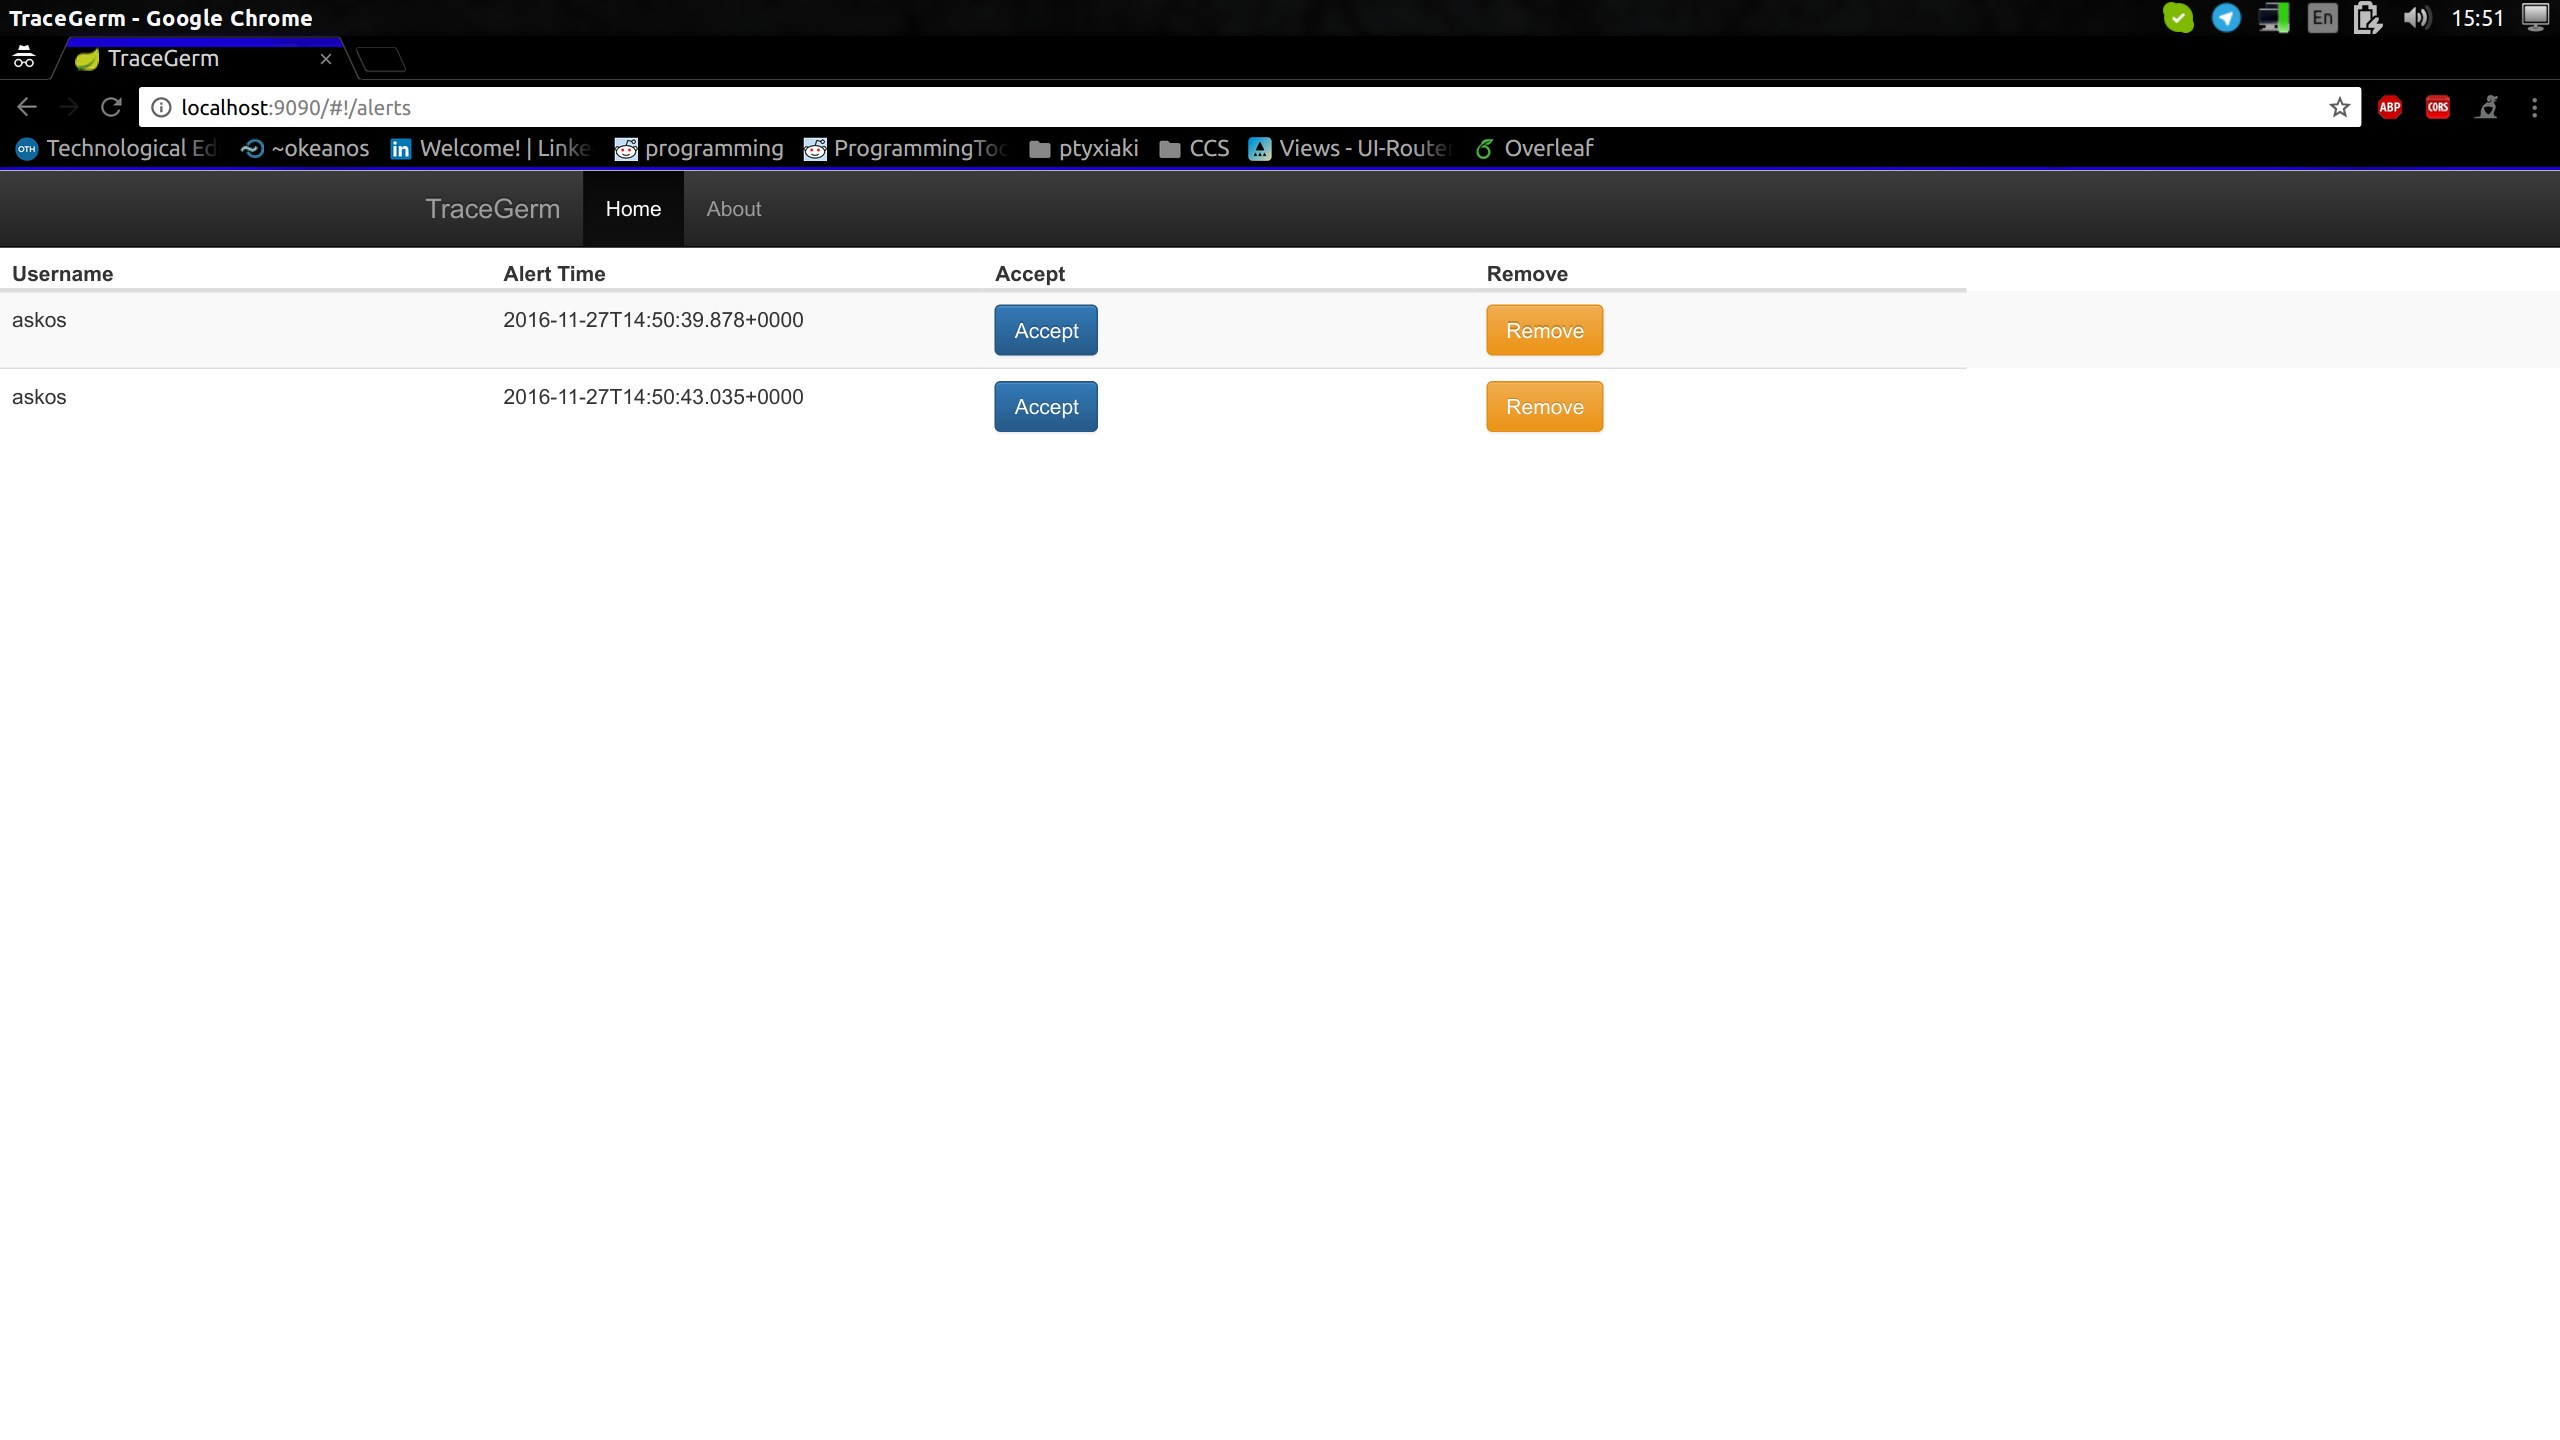
\includegraphics[width=150mm]{images/alerts.png}
  \caption{Εμφάνιση συναγερμών}
  \label{fig:login-webapp}
\end{figure}

\newpage

\section{Web Service}
Παρακάτω θα παρουσιάσουμε λεπτομερώς τα πιο καίρια κομμάτια του εξυπηρετητή. Θα παρουσιάσουμε το μοντέλο της εφαρμογής μας καθώς και τα πιο σημαντικά κομμάτια όπως ο αλγόριθμος αποστολής ειδοποιήσεων στους χρήστες καθώς και οι διαφορετικοί τρόποι επικοινωνίας.

\subsection{Μοντέλο Εφαρμογής}
Το μοντέλο της εφαρμογής αποτελείται από τα αντικείμενα τα οποία κάνουμε χρήση κατά τη διάρκεια εκτέλεσης του συστήματος για να επεξεργαστούμε, εμφανίσουμε και φυσικά να δημιουργήσουμε τα δεδομένα του συστήματος μας. Συγκεκριμένα το μοντέλο της εφαρμογής μας αποτελείτε από τέσσερις βασικές οντότητες. Στο διάγραμμα ~\ref{fig:domain-diagram} μπορούμε να δούμε το βασικό μοντέλο της εφαρμογής.

\begin{figure}[h]
  \centering
  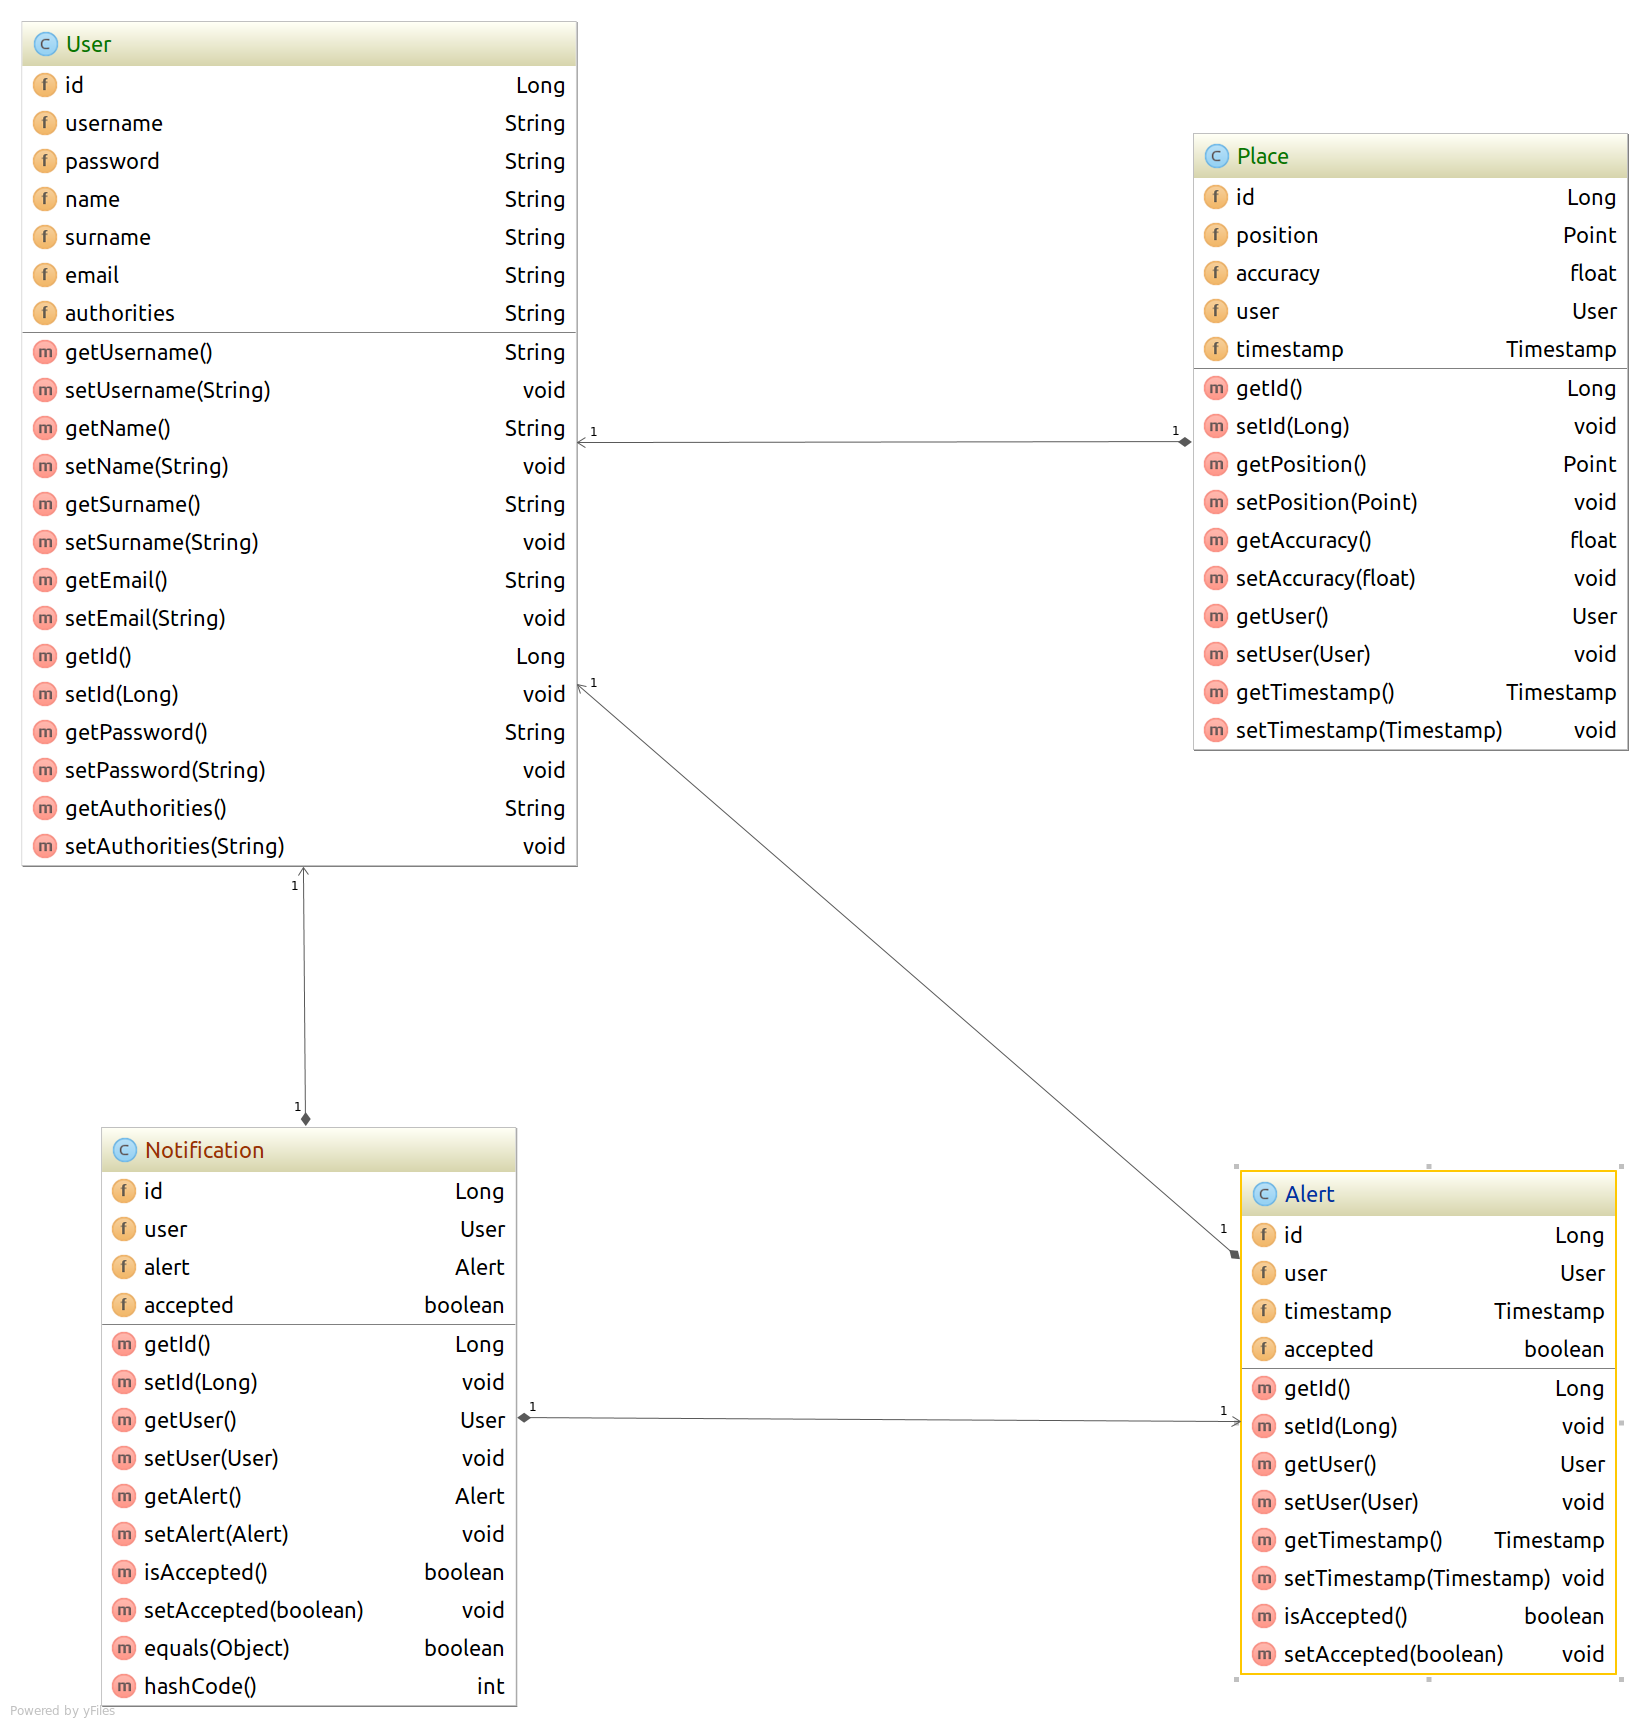
\includegraphics[width=150mm]{images/domain-diagram.png}
  \caption{Μοντέλο εφαρμογής}
  \label{fig:domain-diagram}
\end{figure}

\newpage

\subsection{Επικοινωνία με το API}
Όπως έχουμε προαναφέρει η επικοινωνία των πελατών με τον εξυπηρετητή γίνεται κατά βάση με τη χρήση του ReST API όπως επίσης και με το μοτίβο Publish/Subscribe μέσω του πρωτοκόλλου websockets. Παρακάτω θα παρουσιάσουμε εις βάθος τους δύο παραπάνω τρόπους επικοινωνίας και τις περιπτώσεις χρήσης τους καθώς και τα JSON μηνύματα τα οποία ανταλλάσσονται κατά τη διάρκεια της επικοινωνίας.

\subsection{Rest API}
Ο βασικός τρόπος επικοινωνίας γίνεται μέσω του Rest API. Οι εφαρμογές μας στέλνουν συγκεκριμένα http αιτήματα τα οποία αφού ο εξυπηρετητής μας επεξεργαστεί επιστρέφει την απαραίτητη απάντηση στον πελάτη σε μορφή JSON. Για να γίνει ξεκάθαρη η σύνταξη για την επικοινωνία, παρακάτω θα εμφανίσουμε ένα πραγματικό παράδειγμα από την εφαρμογή μας. 

\subsubsection{Αίτημα πελάτη}
Ο πελάτης δημιουργεί ένα αίτημα για την εύρεση των τελευταίων τοποθεσιών στις οποίες βρέθηκε. Το αίτημα εμφανίζεται στο κώδικα ~\ref{lst:places-request} και παρατηρούμε ότι η εφαρμογή κάνει ένα αίτημα GET αίτημα στο URI: /places/user/lastPlaces.  

\begin{lstlisting}[language=Java, caption=Αίτημα τελευταίων τοποθεσιών του χρήστη, label={lst:places-request}]
getLast10Positions: function () {
      return HttpSecure.get(apiUrl + '/places/user/lastPlaces');
    }
\end{lstlisting}

\subsubsection{Επεξεργασία εξυπηρετητή}
Ο εξυπηρετητής λαμβάνει το αίτημα στο επίπεδο των διαχειριστών όπως φαίνεται στον αλγόριθμο ~\ref{lst:places-controller}. Όταν ο υπεύθυνος διαχειριστής απολάβει το αίτημα φροντίζει να μεταφέρει το αίτημα στο επόμενο επίπεδο, το επίπεδο των υπηρεσιών.

\begin{lstlisting}[language=Java, caption=Διαχειριστής εξυπηρετητή, label={lst:places-controller}]
    
@RepositoryRestController
@RequestMapping("/api/places")
public class PlaceController {

  private final Logger logger = Logger.getLogger(this.getClass());

  @Autowired
  private UserRepository userRepository;

  private final PlaceService placeService;

  private final SecurityContextProvider securityContextProvider;

  @Autowired
  public PlaceController(PlaceService placeService, SecurityContextProvider securityContextProvider) {
    this.placeService = placeService;
    this.securityContextProvider = securityContextProvider;
  }

  @RequestMapping(value = "/user/lastPlaces", method = RequestMethod.GET)
  public ResponseEntity<?> getLast10PlacesByToken() throws AuthenticationException {
    
    User user = this.userRepository
    .findByUsername(securityContextProvider
    .getUserDetails().getUsername());
    
    return ResponseEntity
    .ok(placeService.getLast10Places(user));
  }
}

\end{lstlisting}

Το επίπεδο των υπηρεσιών είναι υπεύθυνο για την οποιαδήποτε επεξεργασία των δεδομένων πριν την αποστολή στο χρήστη. Το επίπεδο υπηρεσιών λαμβάνει τα δεδομένα από το επίπεδο δεδομένων και γίνεται εφαρμογή της λογικής του συστήματός μας όπου αυτό είναι αναγκαίο (Αλγόριθμος ~\ref{lst:places-service}).

\begin{lstlisting}[language=Java, caption=Επίπεδο υπηρεσιών εξυπηρετητή, label={lst:places-service}]
    
@Service
@Transactional
public class PlaceServiceImpl implements PlaceService {

    private final PlaceRepository placeRepository;

    @Autowired
    public PlaceServiceImpl(PlaceRepository placeRepository) {
        this.placeRepository = placeRepository;
    }

    @Override
    public List<Place> getLast10Places(User user) {
        return placeRepository.getLast10PlacesByUserId(user.getId());
    }
}

\end{lstlisting}

Τέλος το επίπεδο δεδομένων φροντίζει για την ανάκτηση των δεδομένων τα οποία ζητήθηκαν από το επίπεδο των υπηρεσιών. Στον αλγόριθμο ~\ref{lst:places-repository} μπορούμε να δούμε το ακριβές ερώτημα που εκτελείται στη βάση δεδομένων.

\begin{lstlisting}[language=Java, caption=Επίπεδο δεδομένων εξυπηρετητή, label={lst:places-repository}]
    
@RepositoryRestResource(collectionResourceRel = "places", path = "places")
public interface PlaceRepository extends JpaRepository<Place, Long> {

    @RestResource(exported = false)
    @Query(value = "select * from places where fk_user = :userId order by  timestamp desc limit 10", nativeQuery = true)
    List<Place> getLast10PlacesByUserId(@Param("userId") Long userId);
    
    

}


\end{lstlisting}

\subsubsection{Δεδομένα επιστροφής}
Έχοντας ολοκληρώσει την επεξεργασία των δεδομένων, αυτά επιστρέφονται στο πελάτη με τη μορφή JSON. Εδώ να αναφέρουμε ότι η αναπαράσταση με τη μορφή JSON δεν είναι η μοναδική που μπορεί να επιλεγεί καθώς θα μπορούσαμε να κάνουμε χρήση της μορφής XML. Παρόλα αυτά στη προκειμένη περίπτωση η μορφή JSON επιλέχθηκε καθώς και οι δύο εφαρμογές πελατών γράφτηκαν με τη γλώσσα JavaScript η οποία καθιστά πιο εύκολη την χρήση της μορφής αυτής.

\begin{lstlisting}[language=Java, caption=Μορφή JSON δεδομένων, label={lst:places-json}]

    "places": [
      {
        "position": {
          "latitude": -71.060316,
          "longitude": 48.432044
        },
        "accuracy": 46,
        "timestamp": "2016-10-23T18:50:30.441+0000"
      },
      {
        "position": {
          "latitude": -71.060316,
          "longitude": 48.432044
        },
        "accuracy": 46,
        "timestamp": "2016-10-23T18:50:30.441+0000"
      },
.....
}
\end{lstlisting}

\subsubsection{ReST API αιτήματα-endpoints}
Παρακάτω θα εμφανίσουμε όλα τα δυνατά αιτήματα τα οποία μπορούν να χρησιμοποιηθούν για την επικοινωνία των πελατών με τον εξυπηρετητή, τα αποκαλούμενα endpoints. Κάθε αίτημα θα παρουσιαστεί με την αντίστοιχη http μέθοδο καθώς επίσης και μία μικρή περιγραφή.

\begin{itemize}
\item \textbf{GET /api/alerts/\{id\}}  \newline
Λήψη πληροφοριών για ένα συγκεκριμένο συναγερμό

\item \textbf{DELETE /api/alerts/\{id\}}  \newline
Διαγραφή ενός συγκεκριμένου συναγερμού

\item \textbf{POST /api/alerts/} \newline
Δημιουργία ενός καινούριου συναγερμού

\item \textbf{PUT /api/alerts/\{id\}}  \newline
Eπεξεργασία ενός συγκεκριμένου συναγερμού

\item \textbf{GET /api/alerts/isAccepted/false} \newline
Λήψη όλων των συναγερμών οι οποίοι δεν έχουν γίνει αποδεκτοί ακόμη

\item \textbf{GET /api/notifications/user/notAcceptedNotifications} \newline
Λήψη όλως των ειδοποιήσεων ενός χρήστη

\item \textbf{PUT /api/notifications/\{id\}} \newline
Επεξεργασία μίας συγκεκριμένης ειδοποίησης

\item \textbf{GET /api/places/user/lastPlaces} \newline
Εύρεση τελευταίων τοποθεσιών ενός χρήστη

\item \textbf{POST /api/places} \newline
Δημιουργία μίας νέας καταγραφής τοποθεσίας

\item \textbf{POST /api/users} \newline
Δημιουργία ενός νέου χρήστη

\item \textbf{PUT /api/users/\{id\}} \newline
Επεξεργασία ενός χρήστη

\item \textbf{GET /api/auth} \newline
Λήψη στοιχείων χρήστη που έχει κάνει είσοδο στην εφαρμογή

\item \textbf{POST /api/auth} \newline
Αίτημα επικύρωσης χρήστη

\item \textbf{POST /api/auth/admin} \newline
Αίτημα επικύρωσης υπηρεσιών υγείας
\end{itemize}

\subsection{Publish/Subscribe Websockets}
 Για την παραλαβή δεδομένων σε πραγματικό χρόνο από τους πελάτες μας, έγινε η χρήση του πρωτοκόλλου websockets και του πρότυπου publish/subscribe. Ο εξυπηρετητής αναμένει από τους πελάτες να συνδεθούν (Αλγόριθμος ~\ref{lst:websocket-config}), έπειτα μέσω του websocket ο πελάτης κάνει εγγραφή στα θέματα τα οποία τον απασχολούν και αναμένει για δεδομένα από τον εξυπηρετητή. 
 
 \begin{lstlisting}[language=Java, caption=Βασική ρύθμιση websocket, label={lst:websocket-config}]

@Configuration
@EnableWebSocketMessageBroker
public class WebSocketConfig extends AbstractWebSocketMessageBrokerConfigurer {

    @Override
    public void configureMessageBroker(MessageBrokerRegistry config) {
        config.enableSimpleBroker("/topic");
        config.setApplicationDestinationPrefixes("/app");
    }

    @Override
    public void registerStompEndpoints(StompEndpointRegistry registry) {
        registry.addEndpoint("/api/tracegerm-websocket")
        .setAllowedOrigins("*").withSockJS();
    }

}
\end{lstlisting}

\subsubsection{Δημοσίευση δεδομένων σε ένα θέμα}
Για να γίνει πλήρως κατανοητός ο τρόπος δημοσίευσης δεδομένων με το πρότυπο publish/subscribe μπορούμε να δούμε τον αλγόριθμο  ~\ref{lst:websocket-publish}. Παρατηρούμε λοιπόν ότι δημοσιεύουμε τις ειδοποιήσεις σύμφωνα με το όνομα χρήστη με αποτέλεσμα ο κάθε χρήστης να λαμβάνει μονάχα τις ειδοποιήσεις του και όχι των υπολοίπων.

 \begin{lstlisting}[language=Java, caption=Δημοσίευση ειδοποιήσεων, label={lst:websocket-publish}]

@Service
@Transactional
public class NotificationServiceImpl implements NotificationService {

    private final NotificationRepository notificationRepository;

    private final PlaceRepository placeRepository;

    private final MessageSendingOperations<String> messagingTemplate;

    @Autowired
    public NotificationServiceImpl(NotificationRepository notificationRepository, PlaceRepository placeRepository,
                                   MessageSendingOperations<String> messagingTemplate) {
        this.notificationRepository = notificationRepository;
        this.placeRepository = placeRepository;
        this.messagingTemplate = messagingTemplate;
    }

...

    @Override
    public void sendUserNotifications(List<Notification> notifications) {
        for(Notification notification : notifications) {
            this.messagingTemplate
            .convertAndSend("/topic/notifications/"
            +notification.getUser().getUsername(), notification);
        }
    }

...
}
\end{lstlisting}

\section{Βάση δεδομένων}
Η βάση δεδομένων είναι το κατώτερο κομμάτι του συστήματος μας. Παρακάτω θα παρουσιάσουμε το μοντέλο των δεδομένων μας και θα αναλύσουμε κάποια σημαντικά ερωτήματα τα οποία κάνουν χρήση της επέκτασης PostGIS.


\subsection{Μοντέλο Δεδομένων}
Το μοντέλο δεδομένων αποτελείται από τους πίνακες τους οποίους χρησιμοποιούμε για την αποθήκευση των δεδομένων μας. Στο διάγραμμα ~\ref{fig:db-diagram} μπορούμε να δούμε όλους τους πίνακες που χρησιμοποιούμε για τα δεδομένα μας. Εδώ αξίζει να αναφερθούμε στο πίνακα τον οποίο καταγράφουμε τις τοποθεσίες του χρήστη. Παρατηρούμε λοιπόν πως σε αντίθεση με τους υπόλοιπους πίνακες, ο συγκεκριμένος έχει μια στήλη η οποία διατηρεί τα γεωγραφικά πλάτη και μήκη μια τοποθεσίας σε τύπο Geometry ο οποίος προέρχεται από την επέκταση PostGIS.

\begin{figure}[h]
  \centering
  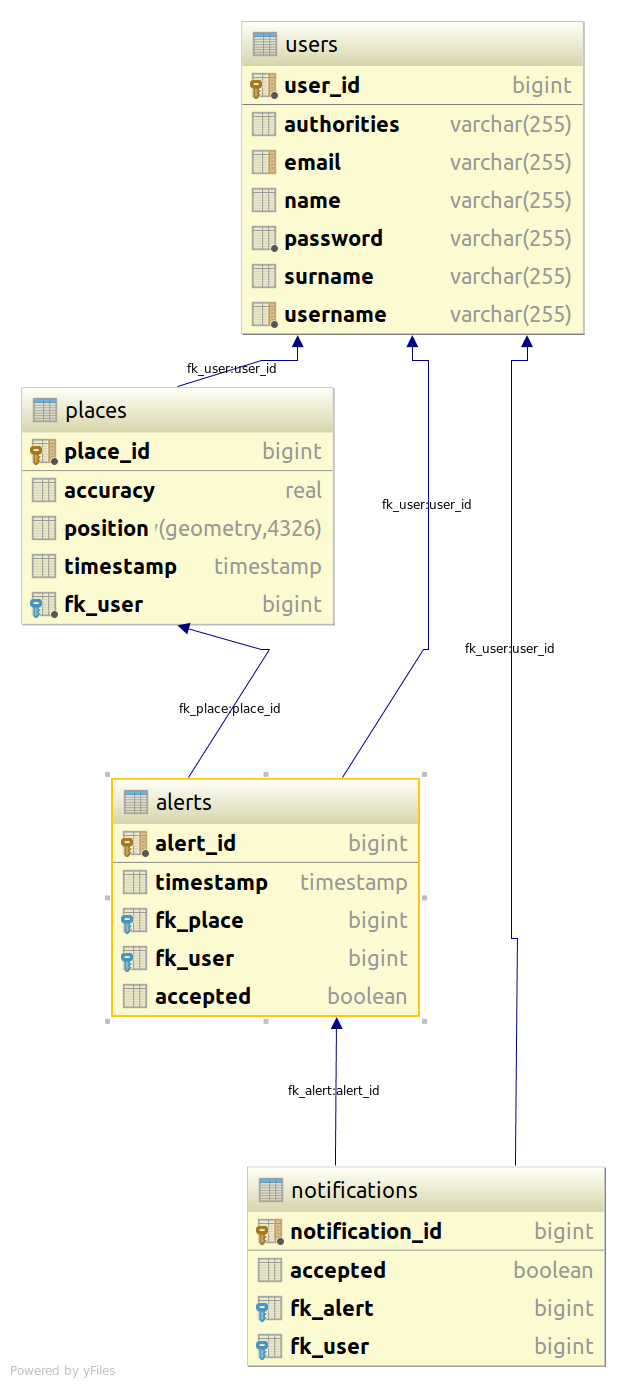
\includegraphics[width=100mm]{images/db-diagram.png}
  \caption{Μοντέλο δεδομένων}
  \label{fig:db-diagram}
\end{figure}

\clearpage

\subsection{Σύνθετα ερωτήματα}
Τέλος ένα σημείο το οποίο θα πρέπει να παραμείνουμε είναι ο τρόπος ανάκτησης δεδομένων από την επέκταση PostGIS. Παρακάτω στον αλγόριθμο ~\ref{lst:sql-query} βλέπουμε το ερώτημα το οποίο μας επιστρέφει τους χρήστες οι οποίοι βρέθηκαν στο ίδιο σημείο με κάποιο χρήστη ο οποίος έστειλε ένα συναγερμό, σε μία διάμετρο δέκα μέτρων καθώς επίσης και σε ένα συγκεκριμένο χρονικό διάστημα. 
\par
Το ερώτημα φαίνεται ιδιαίτερα απλό παρόλα αυτά χωρίς τη χρήση της επέκτασης PostGIS θα ήταν αδύνατο χωρίς τη δημιουργία πολυσύνθετων μεθόδων στη βάση δεδομένων ή στον εξυπηρετητή.

 \begin{lstlisting}[language=SQL, caption=Σύνθετο ερώτημα τοποθεσιών, label={lst:sql-query}]

select * from places p, users u where st_point_inside_circle(p.position,:longitude,:latitude,10) and p.timestamp between to_timestamp(:fromTime, 'YYYY/MM/DD hh24:mi:ss') and to_timestamp(:fromTime, 'YYYY/MM/DD hh24:mi:ss') + interval '10 minutes' and p.fk_user != :userId and p.fk_user = u.user_id;
            
\end{lstlisting}
\chapter{Έλεγχος Ποιότητας}

\section{Εισαγωγή}
Καθώς το σύστημα μας μεγαλώνει συνεχώς και οι έννοιες γίνονται όλο και πιο σύνθετες οφείλουμε να ελέγχουμε αν όλες οι λειτουργίες δουλεύουν όπως αναμένουμε. Για να γίνει αυτό δημιουργήθηκαν test στα επιμέρους συστήματα για τον έλεγχο των διάφορων κομματιών του κώδικά μας. Παρακάτω θα παρουσιάσουμε τα εργαλεία που χρησιμοποιήθηκαν όπως επίσης και μερικά παραδείγματα για να γίνει ξεκάθαρος ο τρόπος με τον οποίο ελέγχθηκε η λειτουργικότητα του συστήματος.

\section{Unit Testing}
Μία από τις πιο βασικές έννοιες στον έλεγχο ποιότητας είναι το Unit Testing. Σκοπός των unit tests είναι ο έλεγχος λειτουργίας ενός συγκεκριμένου κομματιού κώδικα και τις λογικής την οποία αυτό εκφράζει. Έτσι δημιουργείτε μια απομόνωση των διάφορων λειτουργιών και ο έλεγχος τους γίνεται πιο εύκολος. Παρακάτω θα αναφερθούμε στα εργαλεία που χρησιμοποιήθηκαν για τη δημιουργία unit tests στις εφαρμογές μας καθώς και στον εξυπηρετητή.

\subsection{Εφαρμογές}
Όπως έχουμε προαναφέρει, η εφαρμογή κινητών συσκευών καθώς και η διαδικτυακή εφαρμογή αναπτύχθηκαν με τη χρήση του Angular framework. Το Angular framework έχει γραφτεί έχοντας κατά νου τις βασικές αρχές του ελέγχου ποιότητας. Έτσι υπάρχουν εργαλεία τα οποία βοηθούν στη δημιουργία test, όπως το Jasmine framework. 

\subsubsection{Jasmine Framework}
Το Jasmine framework έχει ως γνώμονα τη συμπεριφορά που αναμένεται κατά της διάρκεια του ελέγχου του κώδικα (behavior-driven) έτσι διευκολύνει τη δημιουργία των test. Για να γίνει αυτό αντιληπτό παρακάτω θα παρουσιάσουμε ένα απλό test στο οποίο ελέγχουμε αν ο αλγόριθμος της κρυπτογράφησης των δεδομένων του χρήστη συμπεριφέρεται όπως αναμένουμε.

\begin{lstlisting}[language=Java, caption=Jasmine test, label={lst:jasmine-test}]
describe('LoginController', function() {
  beforeEach(module('tracegerm'));
  var $controller;

  beforeEach(inject(function(_$controller_){
    $controller = _$controller_;
  }));

  describe('#DoEncryption', function() {
    it('checks the encryption', function() {
      var $scope = {};
      var controller = $controller('LoginController', { $scope: $scope });
      $scope.registerInfo.password = 'longerthaneightchars';

      var value = "value";
      var encryptedvalue = $scope.encryptValue(value);
      var text = CryptoJS.AES.decrypt(encryptedvalue.toString(), 
      $scope.registerInfo.password).toString(CryptoJS.enc.Utf8);
      
      expect(value).toEqual(text);
    });
  })
});
\end{lstlisting}

\section{Εξυπηρετητής}
Εφόσον ο εξυπηρετητής έχει γραφθεί με τη γλώσσα Java δημιουργήσαμε test για τον έλεγχο ποιότητας με το JUnit framework.

\subsubsection{Junit Framework}
Το JUnit framework είναι ίσως το πιο διαδεδομένο εργαλείο ελέγχου ποιότητας στη γλώσσα Java. Όπως κάθε εργαλείο για unit testing έχει σαν στόχο τον έλεγχο ενός βασικού μέρους του κώδικα και να συγκρίνει το αποτέλεσμα με τα δεδομένα με τα οποία αναμένουμε. Παρακάτω θα εμφανίσουμε ένα απλό παράδειγμα test στο οποίο ελέγχουμε αν ανακτούμε μονάχα τους συναγερμούς ενός χρήστη οι οποίοι δεν έχουν γίνει ακόμα αποδεκτοί.

\begin{lstlisting}[language=Java, caption=JUnit test, label={lst:junit-test}]
@ActiveProfiles("test")
@RunWith(SpringJUnit4ClassRunner.class)
@SpringApplicationConfiguration(classes = Application.class)
public class AlertTests {


    @Autowired
    private AlertRepository alertRepository;

    @Autowired
    private UserRepository userRepository;

    @Before
    public void setup() {
        User user = new User();
        user.setUsername("user");
        user.setPassword("user");
        userRepository.save(user);
        Alert alert = new Alert();
        alert.setAccepted(false);
        alert.setUser(user);
        Date date = new Date();
        alert.setTimestamp(new Timestamp(date.getTime()));
        alertRepository.save(alert);

        Alert alert2 = new Alert();
        alert2.setAccepted(true);
        alert2.setUser(user);
        alert2.setTimestamp(new Timestamp(date.getTime()));
        alertRepository.save(alert2);
    }

    @Test
    public void testAlertsNotAccepted() {
        Assert.assertEquals(1, alertRepository.findAlertsByAccepted(false).size());
    }

}
\end{lstlisting}

\subsection{Αποτελέσματα ελέγχου ποιότητας}
Μετά την ολοκλήρωση εκτέλεσης των test τα εργαλεία τα οποία έχουν προαναφερθεί, δημιουργούν μία σειρά από αναφορές. Οι αναφορές αυτές, παρουσιάζουν μία λεπτομερή λίστα των test των οποίων έγινε εκτέλεση καθώς και των αποτελεσμάτων τους. Υπάρχουν πολυάριθμοι τρόποι παρουσίασης των αποτελεσμάτων όπως XML, JSON, HTML κτλ. Στη περίπτωσή μας παράγουμε τα αποτελέσματα σε μορφή HTML καθώς θεωρήθηκε η πιο εύκολα αναγνώσιμη μέθοδος. 	
Συνοψίζοντας, παρακάτω στα διαγράμματα ~\ref{fig:junit-report} και ~\ref{fig:protractor-report} μπορούμε να δούμε με λεπτομέρεια τα αποτελέσματα κάποιων από τα test τα οποία δημιουργήθηκαν για την εφαρμογή μας. 

\begin{figure}[h]
  \centering
  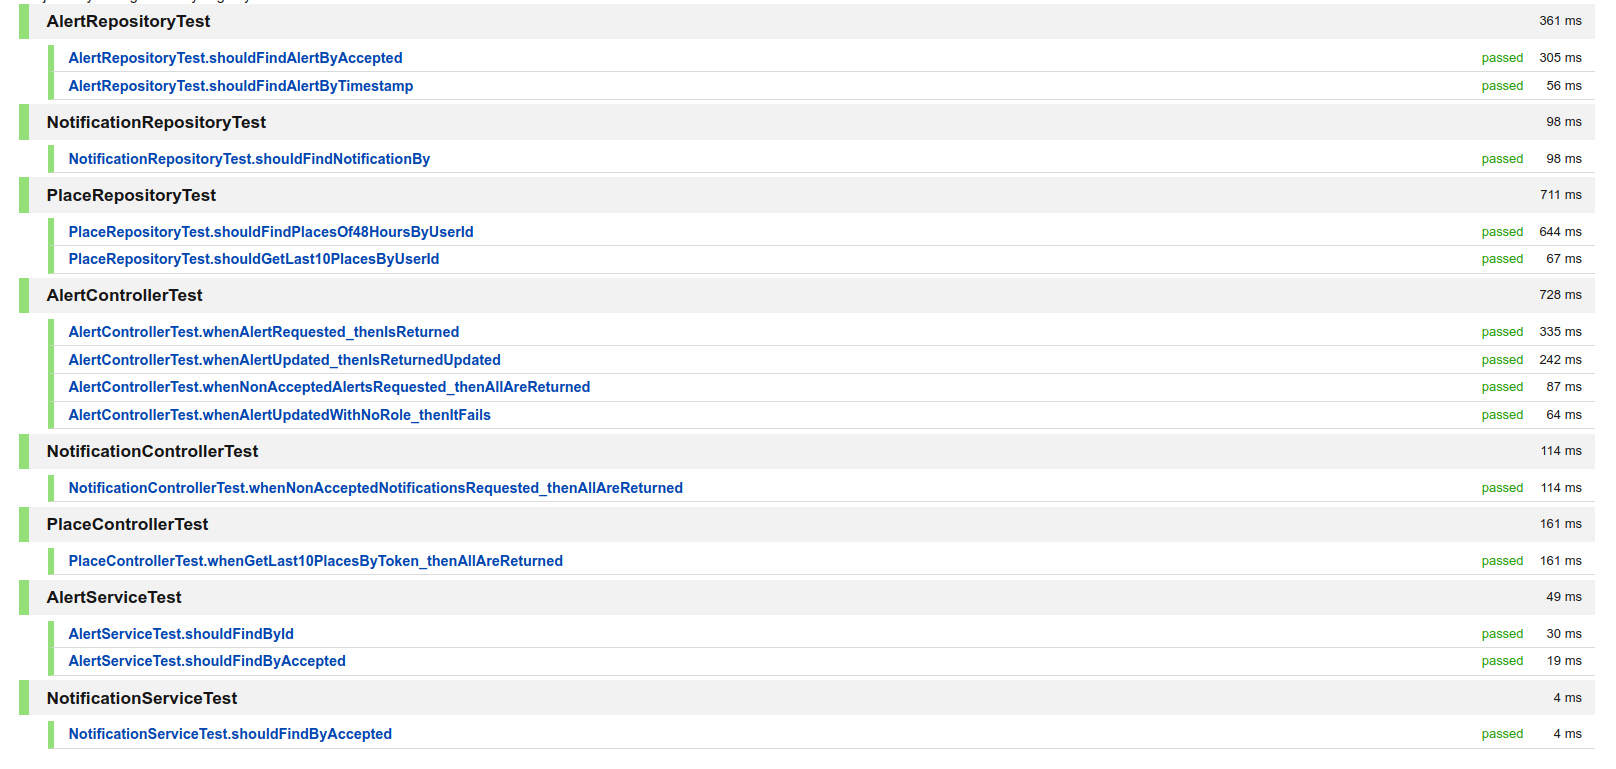
\includegraphics[width=150mm]{images/junit-report.png}
  \caption{Αναφορά Junit}
  \label{fig:junit-report}
\end{figure}

\begin{figure}[h]
  \centering
  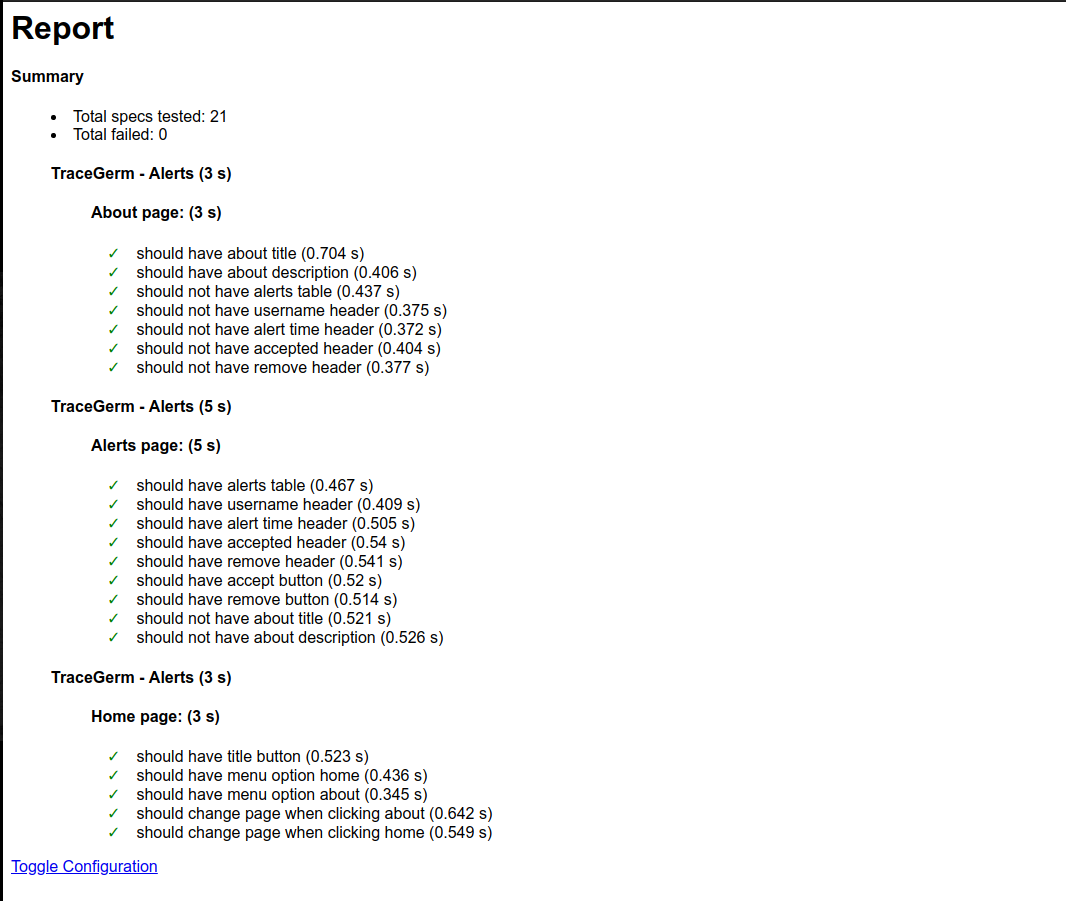
\includegraphics[width=150mm]{images/protractor-report.png}
  \caption{Αναφορά test Εφαρμογών}
  \label{fig:protractor-report}
\end{figure}
\chapter{Επίλογος}
Ο σχεδιασμός και η υλοποίηση ενός τέτοιου συστήματος αποδείχθηκε ένα πολυσύνθετο έργο το οποίο προσέφερε εμπειρία και γνώση σε έναν μεγάλο αριθμό τεχνολογιών \citep{pragmatic}. Παρακάτω θα παρουσιάσουμε τα συμπεράσματα τα οποία προήλθαν για όλα τα επιμέρους κομμάτια του συστήματος μας και των τεχνολογιών οι οποίες χρησιμοποιήθηκαν.


\section{Εφαρμογή κινητών συσκευών}
Βλέποντας πίσω στην επιλογή που έγινε για τη χρήση των Ionic και Cordova frameworks για την δημιουργία της εφαρμογής κινητών συσκευών θα τολμούσαμε να πούμε ότι εμπεριείχε ένα μεγάλο ποσοστό ρίσκου το οποίο τελικά αποδείχτηκε στο μεγαλύτερο βαθμό επιτυχές. Θα μπορούσαμε να πούμε πως, οι παραπάνω τεχνολογίες, έχουν ωριμάσει σε τέτοιο βαθμό όπου ένας χρήστης δεν θα μπορούσε να δει καμία διαφορά σε επιδόσεις μεταξύ αυτών και των native εφαρμογών.

\par
Παρόλα αυτά εδώ πρέπει να αναφέρουμε πως εμφανίστηκαν δυσκολίες στο δρόμο. Η κυριότερη δυσκολία η οποία αντιμετωπίσθηκε ήταν η υπηρεσία καταγραφής των τοποθεσιών. Καθώς είναι ένα ιδιαίτερα δύσκολο κομμάτι ανεξαρτήτως πλατφόρμας κινητών συσκευών, η εύρεση μια βιβλιοθήκης η οποία να υποστηρίζει διάφορες πλατφόρμες εξίσου καλά ήταν ιδιαίτερη πρόκληση. 
\par
Ολοκληρώνοντας θα λέγαμε πως οι παραπάνω τεχνολογίες είναι έγκυρες τεχνολογίες για τη δημιουργία τέτοιων εφαρμογών παρόλα αυτά πάντα υπάρχει χώρος για βελτίωση. Νέες βιβλιοθήκες κάνουν την εμφάνιση τους καθημερινά και προσπαθούν να επιλύσουν θέματα όπως το παραπάνω.

\section{Διαδικτυακή εφαρμογή}
Η χρήση του AngularJS framework για τη δημιουργία της διαδικτυακής εφαρμογής έδειξε την τρομερή εξέλιξη των τεχνολογιών στο τομέα αυτό. Είδαμε πως πλέον η δημιουργία μιας διαδικτυακής εφαρμογής η οποία δίνει στο χρήστη την αίσθηση και τις επιδόσεις μια εφαρμογής υπολογιστών είναι ζωτικής σημασίας. Το AngularJS framework είναι ένα από τις πιο διαδεδομένες τεχνολογίες και πιο ώριμες στο τομέα αυτό. 

\section{Εξυπηρετητής}
Καθώς ο εξυπηρετητής μας έπρεπε να προσφέρει υπηρεσίες σε πολλαπλούς πελάτες η κατασκευή του ήταν ιδιαίτερα δύσκολη από την αρχή. Με τη βοήθεια του Spring framework καθώς και άλλων εργαλείων καταφέραμε να δημιουργήσουμε έναν εξυπηρετητή ο οποίος ανταποκρίνεται στα πρότυπα της αγοράς εργασίας. 

\section{Βάση δεδομένων}
Ένα από τα πιο ιδιαίτερα κομμάτια του συστήματος μας ήταν η βάση δεδομένων. Η ανάγκη αποθήκευσης γεωγραφικών δεδομένων, έφερε την ανάγκη εύρεσης εργαλείων τα οποία καθιστούν δυνατή μια τέτοια διαδικασία. Ύστερα από μελέτη διαφόρων λύσεων, τελικά είδαμε πως η βάση δεδομένων Postgress και η επέκταση PostGIS, ήταν η καλύτερη επιλογή. 

\par
Μέσα από την παραπάνω επιλογή έγινε η πρώτη επαφή με τεχνολογίες αυτού του είδους και παρουσιάστηκε για πρώτη φορά ο μεγάλος βαθμός δυσκολίας και η ιδιαιτερότητα του χώρο των γεωγραφικών δεδομένων. 

\section{Συμπεράσματα}
Βλέποντας το σύστημα μετά την ολοκλήρωση του, παρατηρούμε ότι η δημιουργία του χωρίς την χρήση των προαναφερθέντων framework θα ήταν ιδιαίτερα δύσκολη έως και αδύνατη σε ένα λογικό χρονικό διάστημα. Τα διάφορα προβλήματα τα οποία εμφανίστηκαν επιλύθηκαν μετά από προσωπική έρευνα καθώς και μέσα από την καθοδήγηση του επιβλέποντα καθηγητή. Τέλος η χρήση πολλαπλών framework καθ’ όλη τη διάρκεια της δημιουργίας του συστήματός, μας προσέφερε πολύτιμη εμπειρία για την επαγγελματική εξέλιξη στο χώρο.

\section{Προτάσεις εξέλιξης}
Το σύστημα υλοποιεί στο μεγαλύτερο βαθμό τους αρχικούς στόχους της πτυχιακής εργασίας. Παρ’ όλα αυτά σίγουρα επιδέχεται βελτίωσης και φυσικά περαιτέρω εξέλιξης. Ένα βασικό μέλος του συστήματος το οποίο θα μπορούσε να βελτιωθεί είναι το σύστημα καταγραφής τοποθεσιών στις εφαρμογές κινητών συσκευών. Θα μπορούσε να δοθεί περαιτέρω βαρύτητα στην απόδοση του συστήματος καθώς και στη κατανάλωση ενέργειας από τη μπαταρία της συσκευής. 

\par
Επιπλέον θα μπορούσε να προσφερθεί η δυνατότητα πρόβλεψης της πορείας μίας ασθένειας μέσω εξόρυξης δεδομένων από το σύστημα όπως επίσης και τη χρήση τεχνητής νοημοσύνης. Βέβαια η παραπάνω πρόταση θεωρείται άκρως ιδιαίτερη και ο βαθμός δυσκολίας της την καθιστά ιδιαίτερα δύσκολη να υλοποιηθεί ως πτυχιακή εργασία.

Ο πηγαίος κώδικας όπως και οποιαδήποτε πρόσθετη πληροφορία υπάρχει στην διεύθυνση
https://github.com/TraceGerm.


%Προαιρετικά
\begin{Glossary}
\begin{description}
\item[GPS]Global Positioning System

\item[HTML]HyperText Markup Language

\item[CSS]Cascading Style Sheets

\item[API]Application Programming Interface

\item[ReST]Representational State Transfer

\item[URL]Uniform Resource Locator

\item[JSON]JavaScript Object Notation

\item[TCP]Transmission Control Protocol

\item[SPA]Single Page Application

\item[AES]Advanced Encryption Standard 

\item[URI]Uniform Resource Identifier

\item[XML]Extensible Markup Language

\item[SPA]Single Page Application

\end{description}
\end{Glossary}

\printbibliography

\lastpageinfo
\end{document}
